\begin{abstract}
	On the MSc course "\textit{Computer Modelling Laboratory}" at ELTE, I've worked on a project in nuclear physics, where I studied the behaviour of the Japanese NEBULA detector and its response to neutron bombardment. For the simulation and analysis I've used the Geant4 general-purpose software, which is capable of producing state-of-the-art simulations of particle-matter interactions.
\end{abstract}

\begin{multicols}{2}
\section{Introduction} \label{sec:1}
The NEBULA detector is a plastic scintillator array used to measure positions and momenta of neutrons between $100$ and $300$ MeV with high detection accuracy, large acceptance and sufficient position and velocity resolution\footnote{\url{http://be.nucl.ap.titech.ac.jp/~nebula/}}.

To get a better grasp about the events inside a detector during an experiment - without actually running a neutron experiment - I've created a computer simulation of the NEBULA detector with a more simplified structure in this project. To achieve this, I've used the Geant4 simulation tool, developed for the simulation of the passage of particles through matter.

In this environment I've implemented the NEBULA detector and a neutron beam to shoot at the detector. After the simulation pipeline was ready, I've analysed the spectrum of the detection accuracy and the characteristics of the energy deposition in the detector. I studied the various \texttt{physics list}s in Geant4 and also explored the different type of interacting particles and the physical processes taken place during a simulation. In this report I'll give a thorough summary of all the work I've done on this project during this semester. Since this was a heavily technical project, lot of the sections discuss the raw technical background.

\section{The Geant4 simulation tool} \label{sec:2}
The whole development of the project was done in the environment provided by the Geant4 software, developed by the Geant4 Collaboration at CERN. The user of Geant4 is intended to use it as a simulation engine and develop his or her own software on it. Its immense complexity, the comprehensive list of tools it offers and the way it operates, makes Geant4 an actual
\begin{Figure}
	\centering
	\captionsetup{justification=centering}
	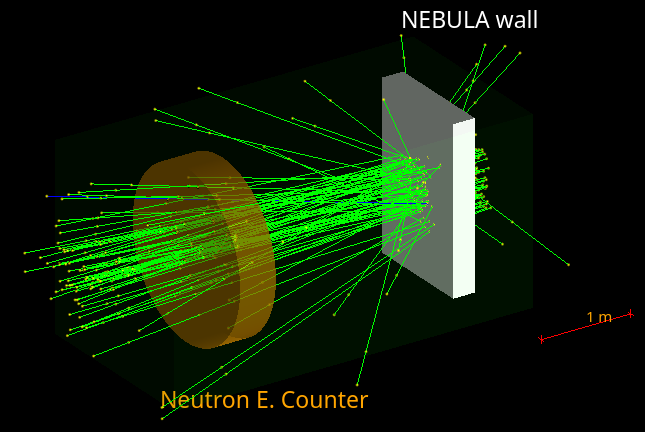
\includegraphics[width=\linewidth]{{images/nebula_3d.png}}
	\captionof{figure}{Geant4 simulation of the transit of 100 neutrons through a section of the NEBULA detector. The wall section of the NEBULA is colored white, while the bluish colored block is an auxiliary neutron energy counter (this latter is not present in case of the real NEBULA detector).} \label{fig:1}
\end{Figure}
\noindent software developing job to use even at the most basic level. Besides the physical simulation capabilities it also offers an OpenGL+Qt backend for visualization, as well as a multi-threading support for both simulation and visualization purposes.

\subsection{Basic concepts}
The structure of a typical Geant4 simulation consist of the detector construction, the particle generation and an event loop. As an addition I've utilized the \texttt{AnalysisManager} module to save the created datasets for further analysis.

In the detector construction we have to define a \texttt{World} geometry, in which all the events of the simulation happens. Anything leaving this volume during any part of the simulation is rendered as non-existent for the time being. Inside the \texttt{World} box we can define other, smaller volumes of arbitrary shapes and sizes, which we can later fill with any predefined, or user-defined material at ease. These volumes will serve as the actual physical objects (targets, detectors, etc.) in a nuclear- or particle physics simulation. The exact detector structure what has been used in the project is discussed in Sec. \ref{sec:3}.

The so called \texttt{particleGun} class was used to create an arbitrary particle beam, shooting neutrons at the create NEBULA detector. In Sec. \ref{sec:4}. I'm discussing about the particle beam in more detail.

\section{Geometry of the NEBULA detector} \label{sec:3}
The NEBULA detector is part of the Japanese SAMURAI beam line system at the RIKEN RI Beam Factory. It consist of $144$ plastic scintillator rods in total, all filled with the BC-$408$ scintillator material, consisting of $52.45\%$ of $H$ and $47.55\%$ of $C$. The rods are distributed equally on the two sides of the beam line with $60$ \texttt{NEUT} rods for neutron detection and $12$ \texttt{VETO} rods to detect charged particles on each side. In the project I only focused on to implement a section of one of the two walls in NEBULA and only the \texttt{NEUT} rods.
\begin{Figure}
	\centering
	\captionsetup{justification=centering}
	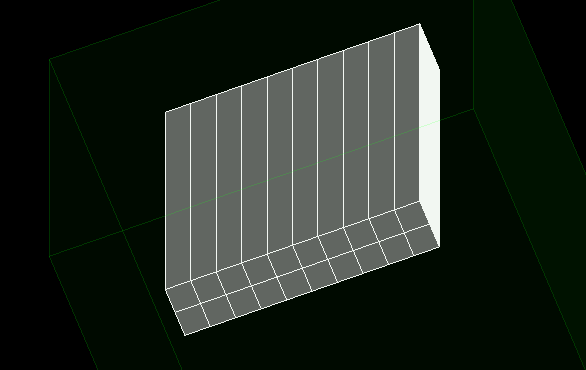
\includegraphics[width=\linewidth]{{images/nebula.png}}
	\captionof{figure}{The structure of the $20$ rods, $2$ layer section of the NEBULA detector viewed from above in the OpenGL+Qt visualization of the Geant4 simulation.} \label{fig:2}
\end{Figure}
On one side of the detector, there are $30-30$ \texttt{NEUT} scintillator rods organized in two layers. Neutrons hit the wall approximately perpendicular and deposits energy as they passes through the scintillator material. To simulate the process of neutron transit through this wall, it is enough to select a small section of it and simulate the bombardment of this part with perpendicular or near-perpendicular neutron beams. For this I've selected a $10$ rods wide (and $2$ rods deep) section of the wall, which I modelled using Geant4. The structure of this geometry can be seen in detail on Fig. \ref{fig:2}.

Parts of the detector construction code was written by Dávid Pesznyák in his 2020 BSc thesis about the calorimetry of muons and neutrons\footnote{\url{http://atomfizika.elte.hu/akos/tezisek/szd/pesznyakdavid_BScszd.pdf}}. This implementation simplifies the NEBULA detector as a square prism, consist of several, smaller, also square prism-shaped scintillator rods. This is already sufficient enough to get approximate simulation results, but it also could be improved later on.

\section{Particle beam} \label{sec:4}
The \texttt{particleGun} class from the Geant4 toolkit allows us to meticulously change every property of the inbound particles in the simulation. In the project I've only configured a neutron particle, and set the starting positions, momenta and energies of the spawned neutrons.

\subsection{Position} \label{ssec:4.1}
Starting positions of the simulated neutrons were sampled from the uniform distribution. Neutrons spawned inside a rectangular area not so far behind the detector wall (marked as \texttt{NEBULA wall} on Fig. \ref{fig:1}.). The rectangle were approximately quarter of the size of the \texttt{NEBULA wall}. The $X$ and $Y$ coordinates (width and height respectively) were randomized, while the $Z$ coordinates (depth) was always at a fix location.

\subsection{Momentum} \label{ssec:4.2}
Similarly to positions, momentum values are also sampled from the uniform distribution. The biggest component in the momenta of particles, points into the direction of the negative $Z$ coordinate axis and guides the particles towards the neighbouring \texttt{NEBULA wall} block. A small inclination is randomly added to each of the particles, which is calculated by generating a uniformly random, small $X$ and $Y$ component for their momentum vector.

\subsection{Energy} \label{ssec:4.3}
The energy range of NEBULA is $100$ - $300$ MeV as in was mentioned in Sec. \ref{sec:1}. To get a detailed picture of this energy interval, I've tested my detector setup with neutrons between $40$ and $360$ MeV in increments of $5$ MeV. This eventually gave a comprehensive view of the detection accuracy of neutrons in the NEBULA detector.

Except for the detection accuracy analysis, all other topics are discussed on a single energy value. The reason for this is, that the change in the initial energies of neutrons (which we fire onto the detector) simply won't change the conclusions that can be drawn from outcome of the analysed effect or measurement. Change in the initial energy usually results in a higher of lower detection rate and a translated distribution for the deposited energy by particles. This is not some peculiar physical effect, so I didn't examined it further.

\section{Data I/O pipeline} \label{sec:5}
Geant4 has no built-in post-processing tools, which means one has to use some other, third-party software to visualize and analyse data accumulated in a simulation. For this, Geant4 offers a versatile I/O library that is able to save any data in the form of XML, CSV or ROOT format.

The \texttt{G4AnalysisManager} is single-handedly responsible for the creation, filling and finally saving the data storing objects in Geant4. In my project work each dataset consisted of $7$ columns and every row represented a simulation step for one specific particle. The created datasets contained the current coordinates of the particle, the deposited energy during the step, the particle type and the physical process currently calculated by Geant4 in the corresponding step, and finally the name of the volume the particle is currently situated in.

\section{Analysis} \label{sec:6}
In my project work, three different topics were examined regarding the NEBULA detector.

The first one was the discover how much energy deposited in each of the detector rods and how does the distribution of the deposited energy values look like.

The second topic focused on the study of the arising particle types and physical processes in the simulation and the proportion of the energy they convey.

The third and the last question was how effective is the simulated segment of the NEBULA detector at the detection of neutrons or energy dissipation in general on different energy levels? The first two topic was discussed on $120$ MeV initial neutron energy, which is in the lower interval of the operation range of the NEBULA detector.

Most figures are only shown for those three physics lists that contain the \texttt{NeutronHP} (\textit{data driven high precision neutron}) package. This package is intended to make simulations of neutron events on lower energies ($<20$ MeV) much more accurate, which comes handy for this project.

\subsection{Distribution of energy deposit} \label{ssec:6.1}
The total energy deposited in the detector rods during the simulation can be easily obtained and then agglomerated from the dataset containing the simulation step-wise measurements. The agglomerated values visualized can be seen on Fig. \ref{fig:4}.  Since the momentum vector of the particles were randomly sampled using an RNG with a set seed, the difference between runs with different physics lists originates purely from the actual difference of the physics lists themselves and from random noise in the simulation.

The kernel density estimation was also calculated with an Epanechnikov kernel for the energies deposited in each simulation steps. 4 out of the 5 tested physics lists produced a similar peak around $2.7$ MeV, while the fifth one (called \texttt{QGSP\_BIC\_HP}) had a similarly shaped, but translated peak at $1.5$ MeV. The two physics list with the \texttt{NeutronHP} package included (\texttt{QGSP\_BERT\_HP} and \texttt{QGSP\_INCLXX\_HP}) resulted in a tightly overlapping and lower peak, while the two other physics lists (\texttt{QBBC} and \texttt{QGSP\_INCLXX}) exhibited a much higher one.

\begin{Figure}
	\centering
	\captionsetup{justification=centering}
	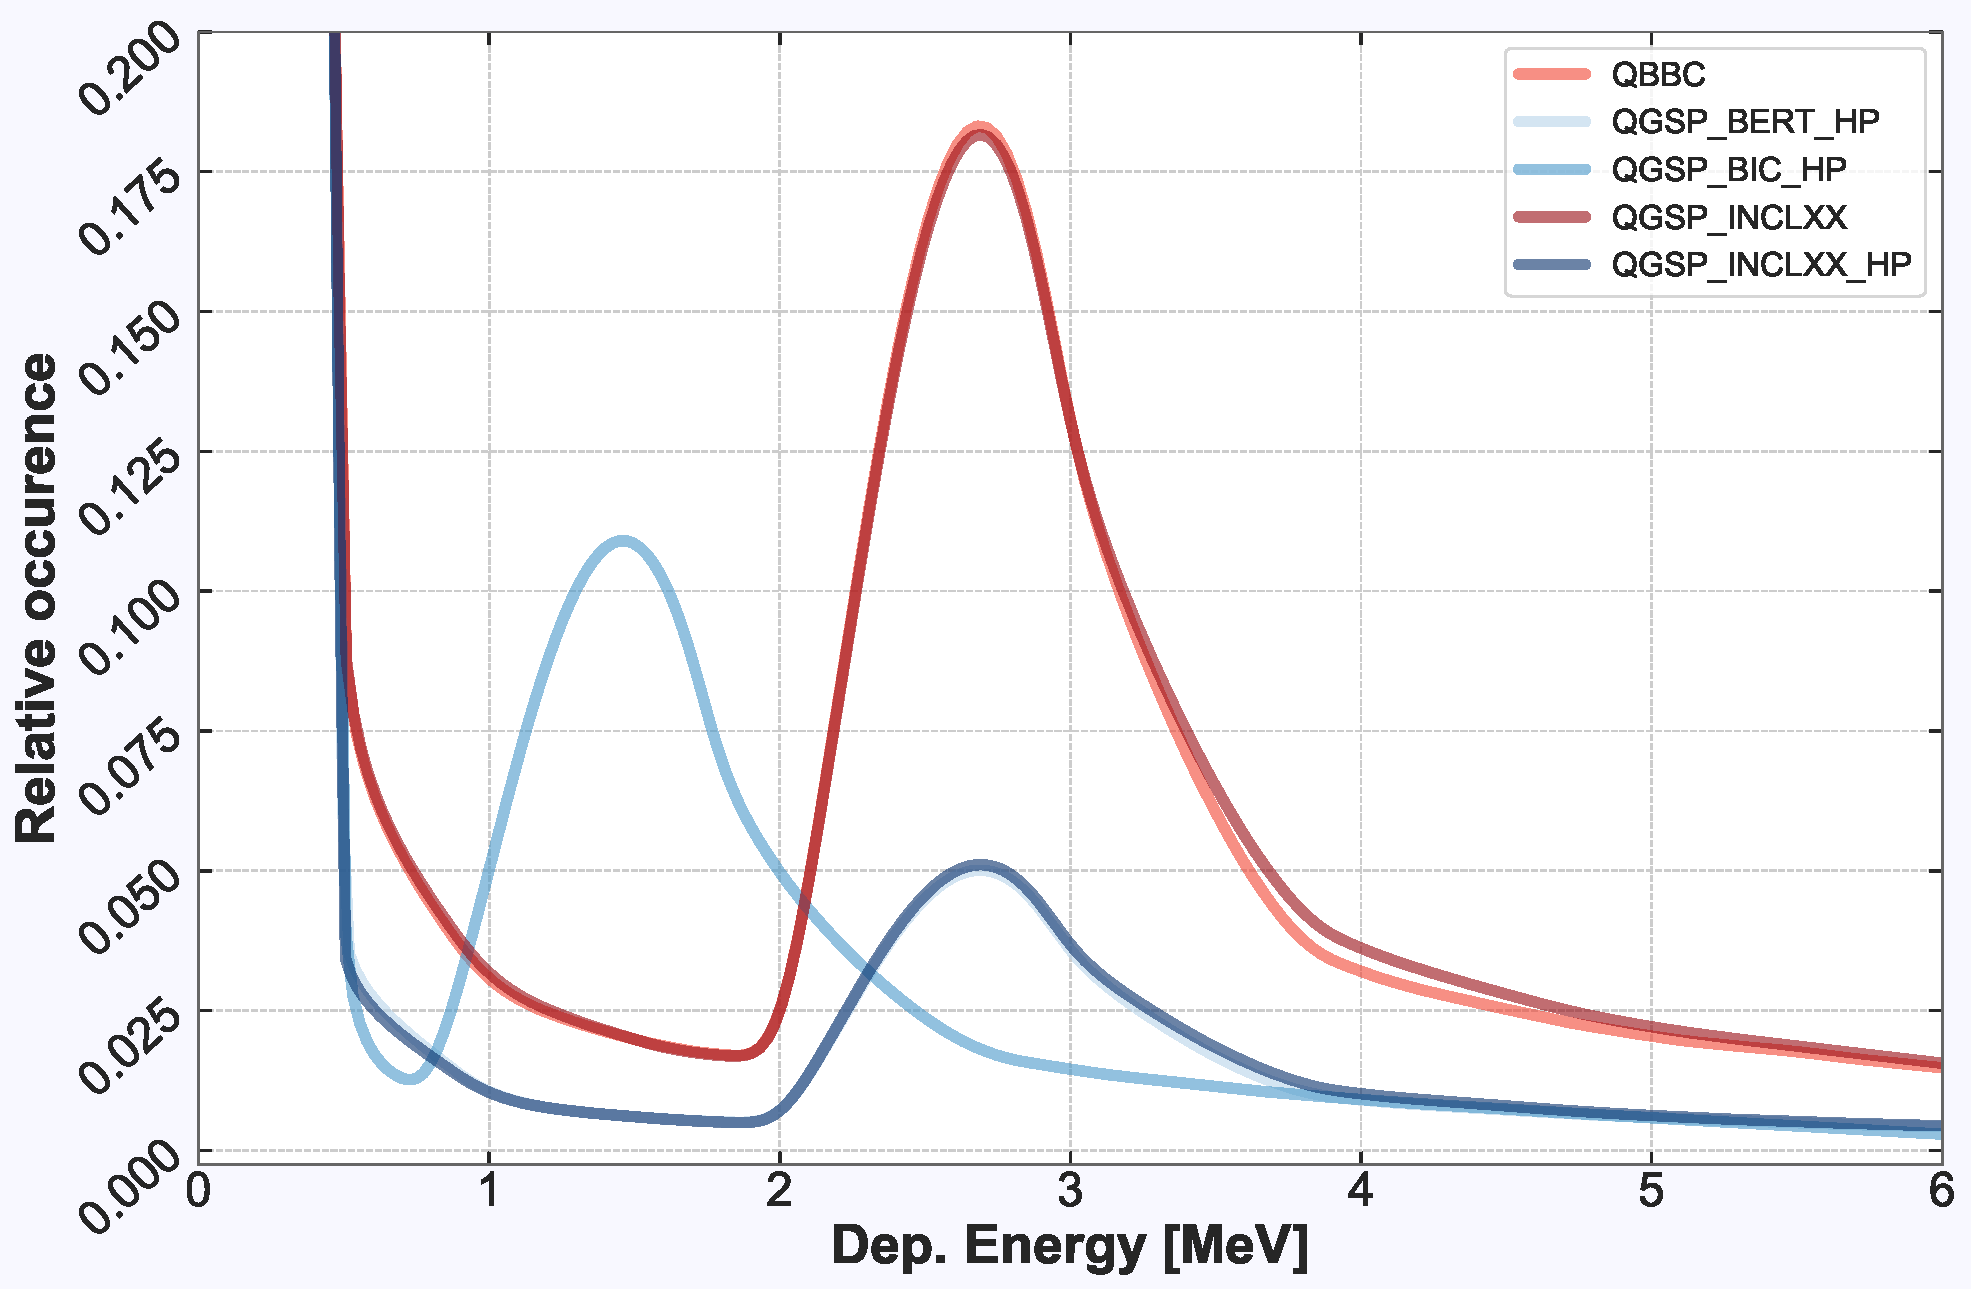
\includegraphics[width=\linewidth]{{images/energy_dist_full_concat_E120.pdf}}
	\captionof{figure}{Kernel density estimation of the energy deposition with an Epanechnikov kernel. Physics list without the \texttt{NeutronHP} package exhibits much larger energy deposition around $2.7$ MeV, than those with the package included. The \texttt{QGSP\_BIC\_HP} however displays unique characteristics, completely separating from the other 4 physics lists.} \label{fig:3}
\end{Figure}

\subsection{Processes and particles} \label{ssec:6.2}
Besides the deposited energy I've also explored the occurrence of different physical processes in the simulation.  What one would see on Fig. \ref{fig:5}. is that the three most frequent events are the energy deposit of hadron ionization (\texttt{hIoni}), the elastic collision of hadrons (\texttt{hadElastic}) and the energy deposit of electron ionization (\texttt{eIoni}).

The processes can be also visualized by their contribution to the total energy deposit. We can see, that for $120$ MeV initial neutron energy, the hadron ionization contributed by far the most to the energy deposition, with ion ionization and electron ionization following it on the second and third places. This distribution is so robust, that it was the very same in case of other physics lists too. These quantities can be seen on \ref{fig:6}.

Similar metrics can be visualized for the particles types taken place in the simulation. On Fig. \ref{fig:7}. the number of simulation steps involving different particle types can be seen. It can be seen, that Geant4 calculated most simulation steps for protons, with neutron on the second place, followed by electrons or photons, depending on the actual physics list used for the simulation. On Fig. \ref{fig:8} one can observe, that most of the energy deposit was made by protons, and where neutrons contribute to almost nothing to it. This can be easily understood by the fact, that most of the energy originates from ionization processes, but neutrons obviously can't be ionized.

\subsection{Detection accuracy and its implications on physics lists} \label{ssec:6.3}
As I've mentioned in Subsec. \ref{ssec:4.3}., data about the NEBULA detector's response to a neutron beam was gathered between $40$ and $360$ MeV. This is also the only topic, where the full, multi-level energy data has been used. In this question we wanted to explore, how effective one segment of the NEBULA detector is in neutron detection, by measuring the detection accuracy for a statistically large enough neutron beam.

I've studied both the neutron and the general energy deposition detection rate in the \texttt{NEUT} rods. Since in a simulated environment we have detailed data of every time step the simulation took, this analysis brakes down to simply sorting the appropriate energy deposit values from the dataset and calculate the proportion of the number of the zero and non-zero energy values (trivially representing no detection and detection respectively). Fig. \ref{fig:9}. shows the general detection rates, while Fig. \ref{fig:10}. shows specifically the neutron detection rates.

On the figure of the total energy distribution in case of 4 out of the 5 different physics lists used, an interesting artifact can be seen around $100$ MeV, where the detection rate drops down by a relatively large amount. From there, the detection accuracy grows and it has a plateau at around $300$ MeV. These values that designates a well-defined section in the dataset coincide with the nominal operating range of the NEBULA detector. In case of the \texttt{QGSP\_BIC\_HP} physics list, none of these effects could be observed. The uniqueness of the \texttt{QGSP\_BIC\_HP} physics list was also observed in case of the discussion of the energy distribution on Fig. \ref{fig:3}.

Focusing solely on the neutron detection rates inside the detector rods, physics list that contain the \texttt{NeutronHP} package produced $100\%$ detection rate n every energy level observed. This is not surprising, since this package is intended to supply the most accurate neutron simulations.

\section{Summary} \label{sec:7}
I used Dávid Pesznyák's BSc thesis from 2020 for reference work throughout my project and tried to recreate his figures as much as possible, while still putting my own contribution and ideas into the project. At the end, I've actually recreated his figures and expanded his work by answering some other interesting questions, like the energy deposition per simulation steps or the detector accuracy.

The topic of the project can be naturally expanded with countless of more in-depth questions regarding the simulation of the NEBULA detector, but to be honest, this was already far more, than enough for this semester.

\end{multicols}

\newpage
\section{Appendix -- Figures}
This appendix contains figures that could not be tastefully inserted into the main corpus. These figures are usually referenced throughout the report.

\subsection{Distribution of energy deposit}
\begin{figure}[htp]
\subfloat[Physics list used : \texttt{QGSP\_BERT\_HP}]{%
  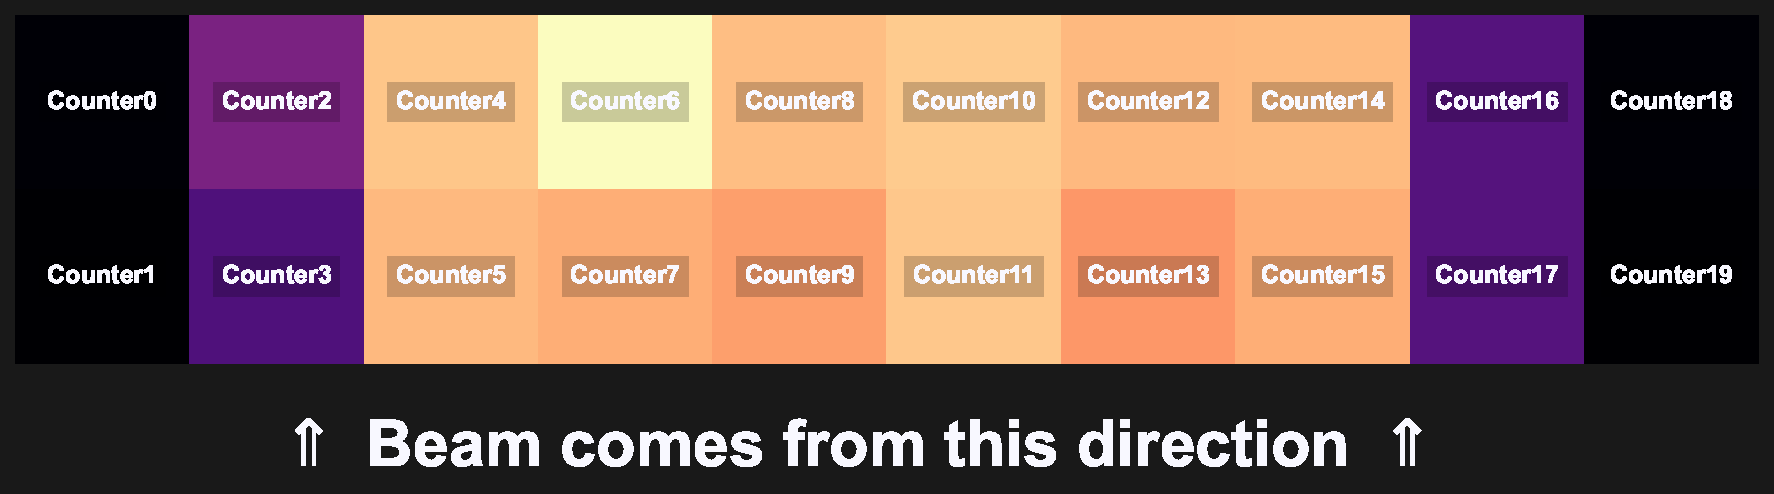
\includegraphics[clip,width=\textwidth]{{images/rod_heatmap_E120_phQGSP_BERT_HP.pdf}}
}

\subfloat[Physics list used : \texttt{QGSP\_BIC\_HP}]{%
  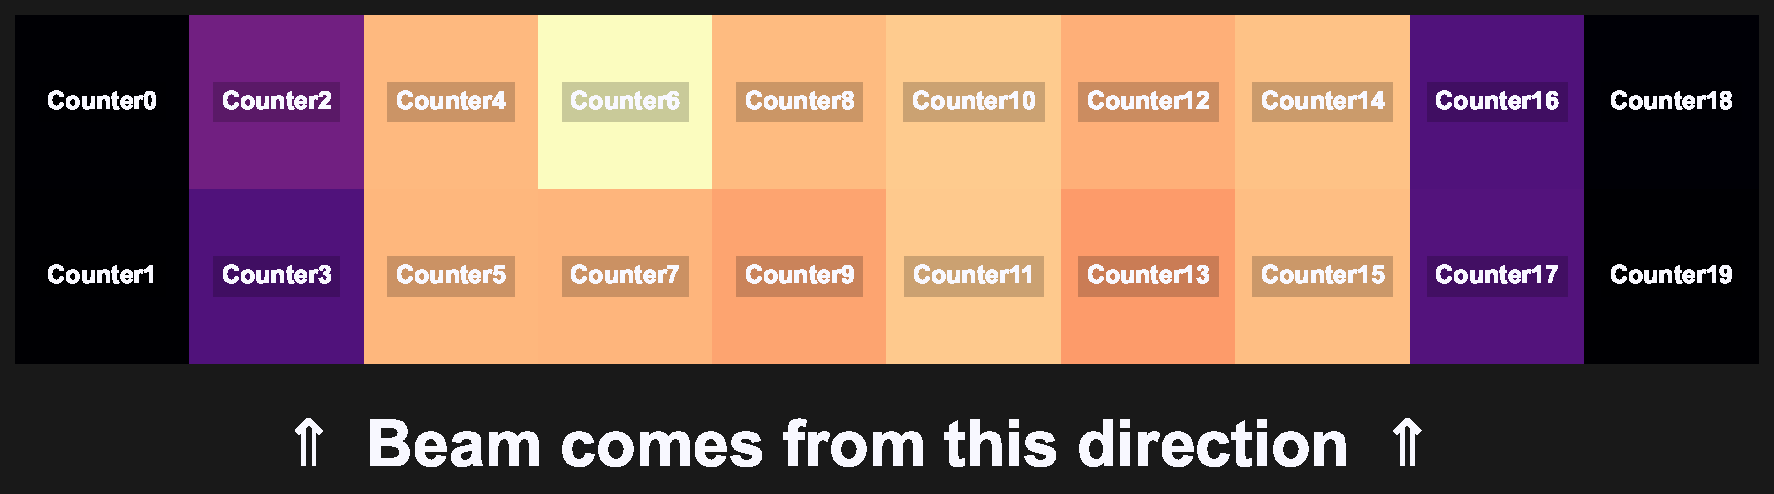
\includegraphics[clip,width=\textwidth]{{images/rod_heatmap_E120_phQGSP_BIC_HP.pdf}}
}

\subfloat[Physics list used : \texttt{QGSP\_INCLXX\_HP}]{%
  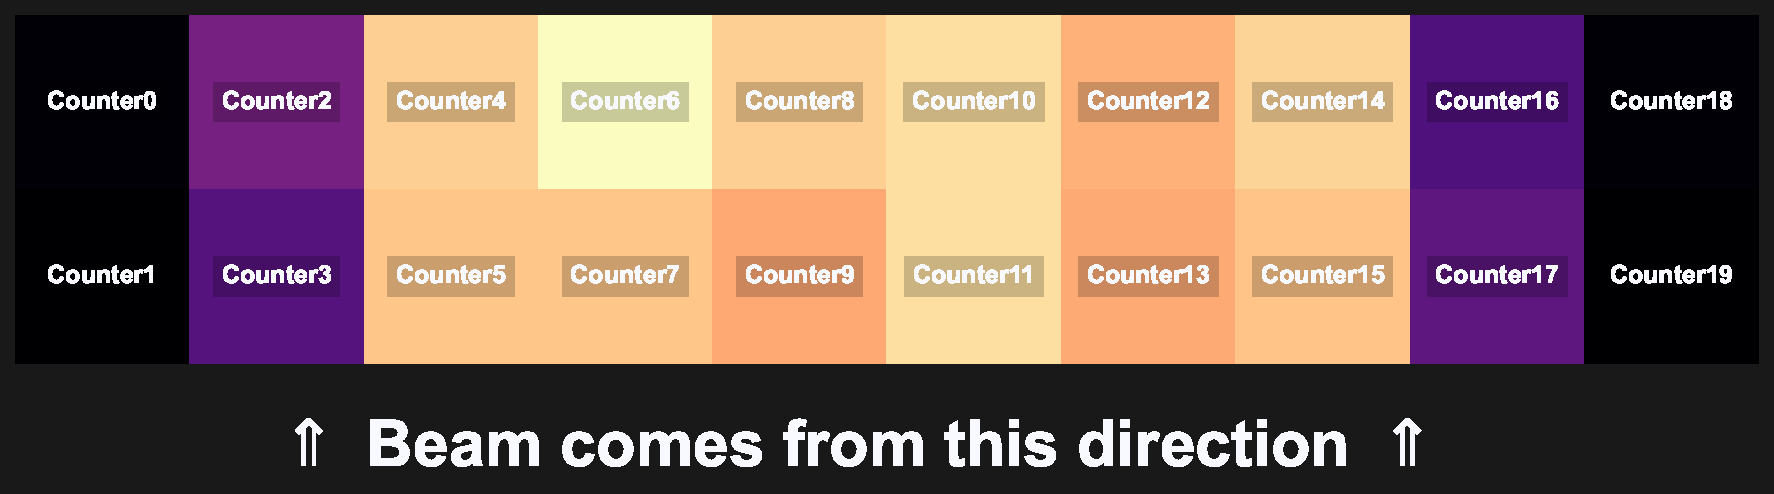
\includegraphics[clip,width=\textwidth]{{images/rod_heatmap_E120_phQGSP_INCLXX_HP.pdf}}
}

\captionof{figure}{Relative distribution of the deposited energy in the \texttt{NEUT} rods of the NEBULA detector for different Geant4 physics lists. The rods are indexed from $0$ to $19$ and coloured by the value of the total energy deposited in them.}\label{fig:4}
\end{figure}

\newpage

\subsection{Processes}
\begin{figure}[htp]
\subfloat[Physics list used : \texttt{QGSP\_BERT\_HP}]{%
  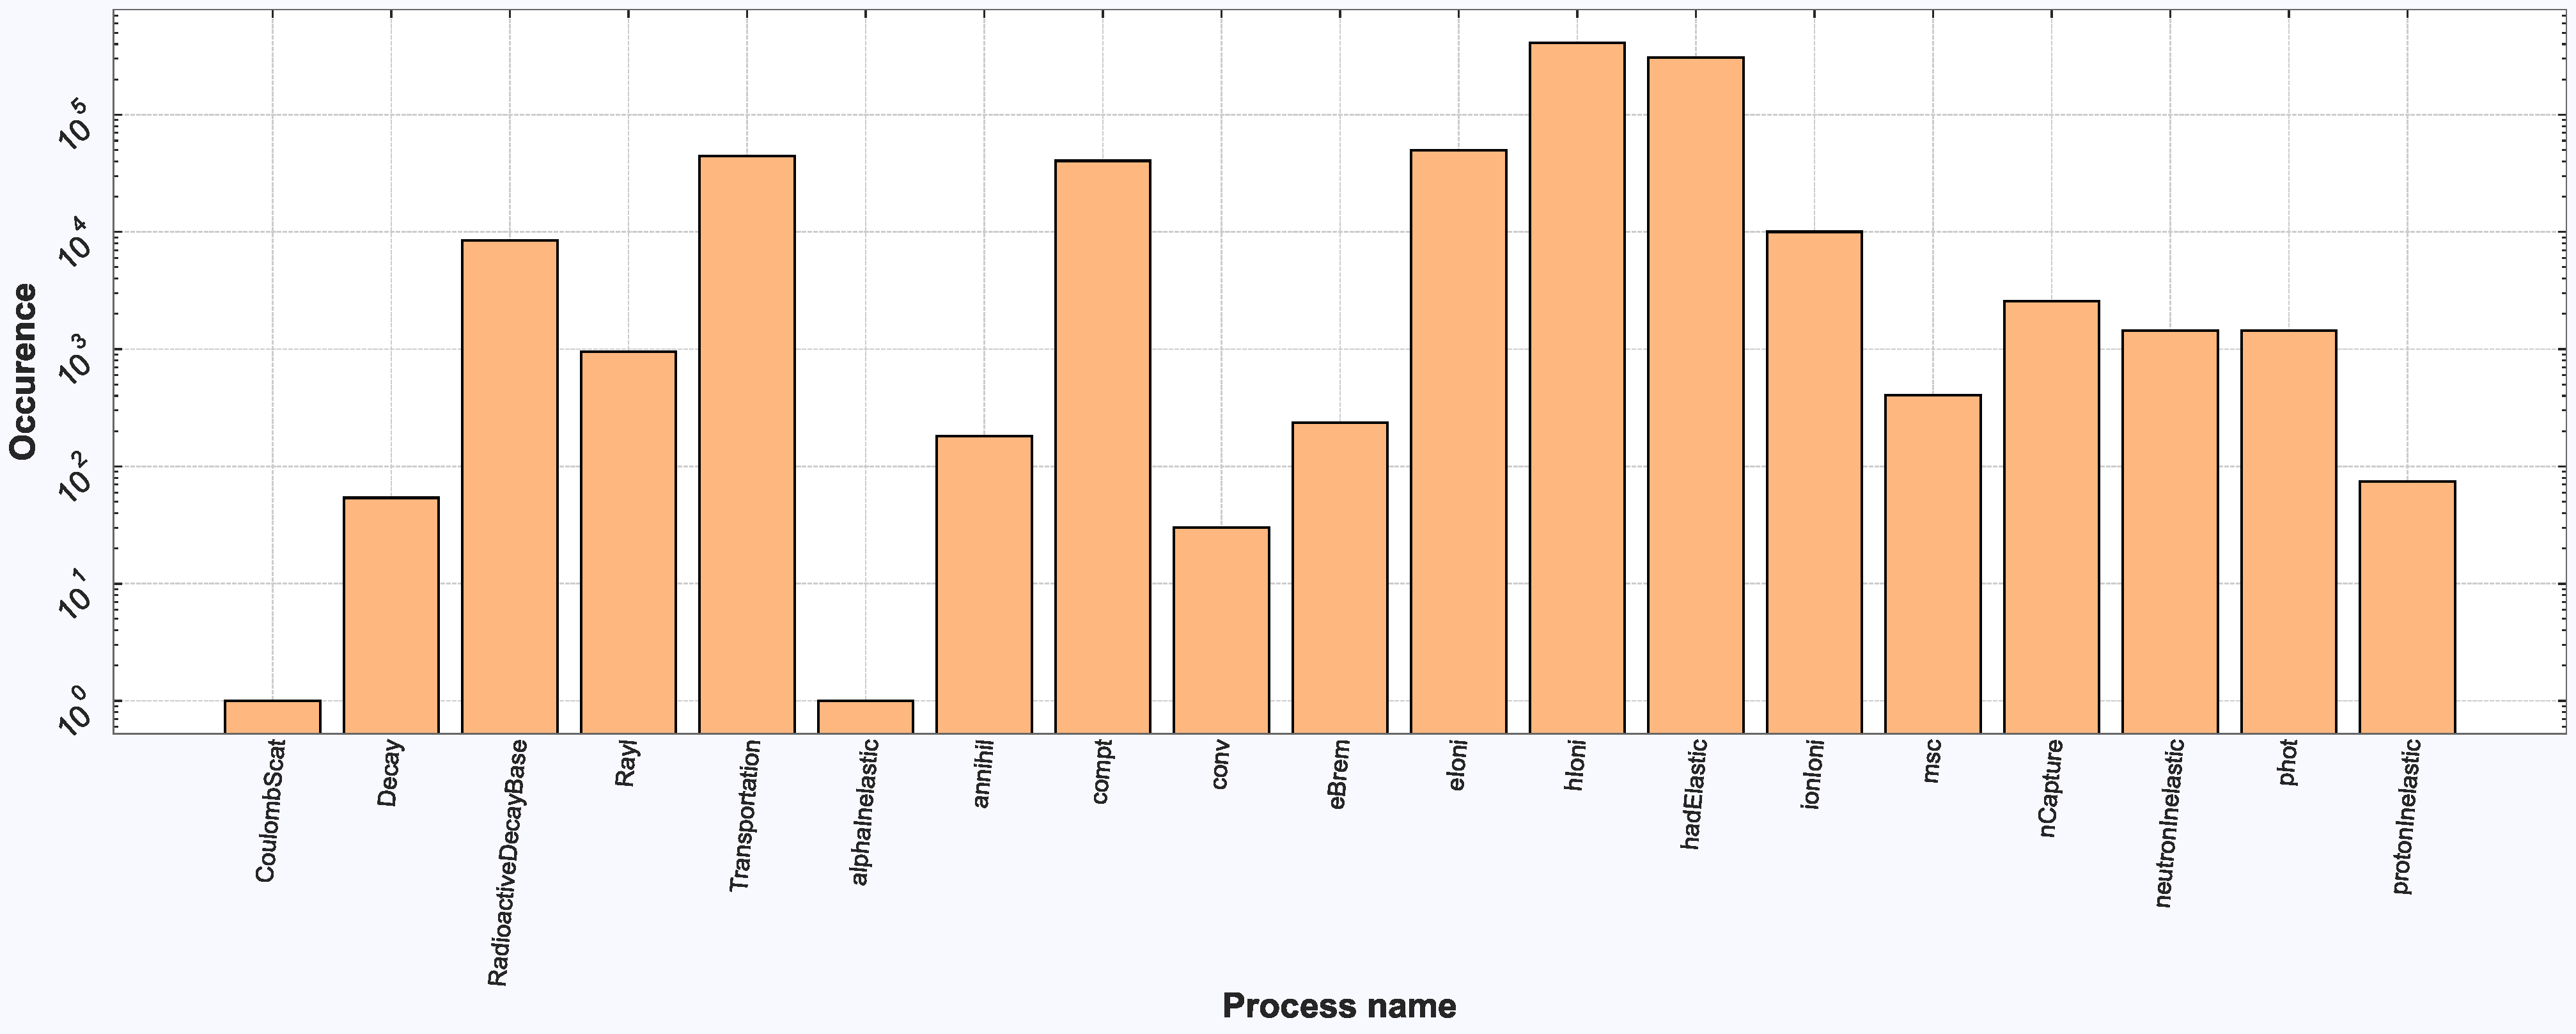
\includegraphics[clip,width=\textwidth]{{images/process_dist_E120_phQGSP_BERT_HP.pdf}}
}

\subfloat[Physics list used : \texttt{QGSP\_BIC\_HP}]{%
  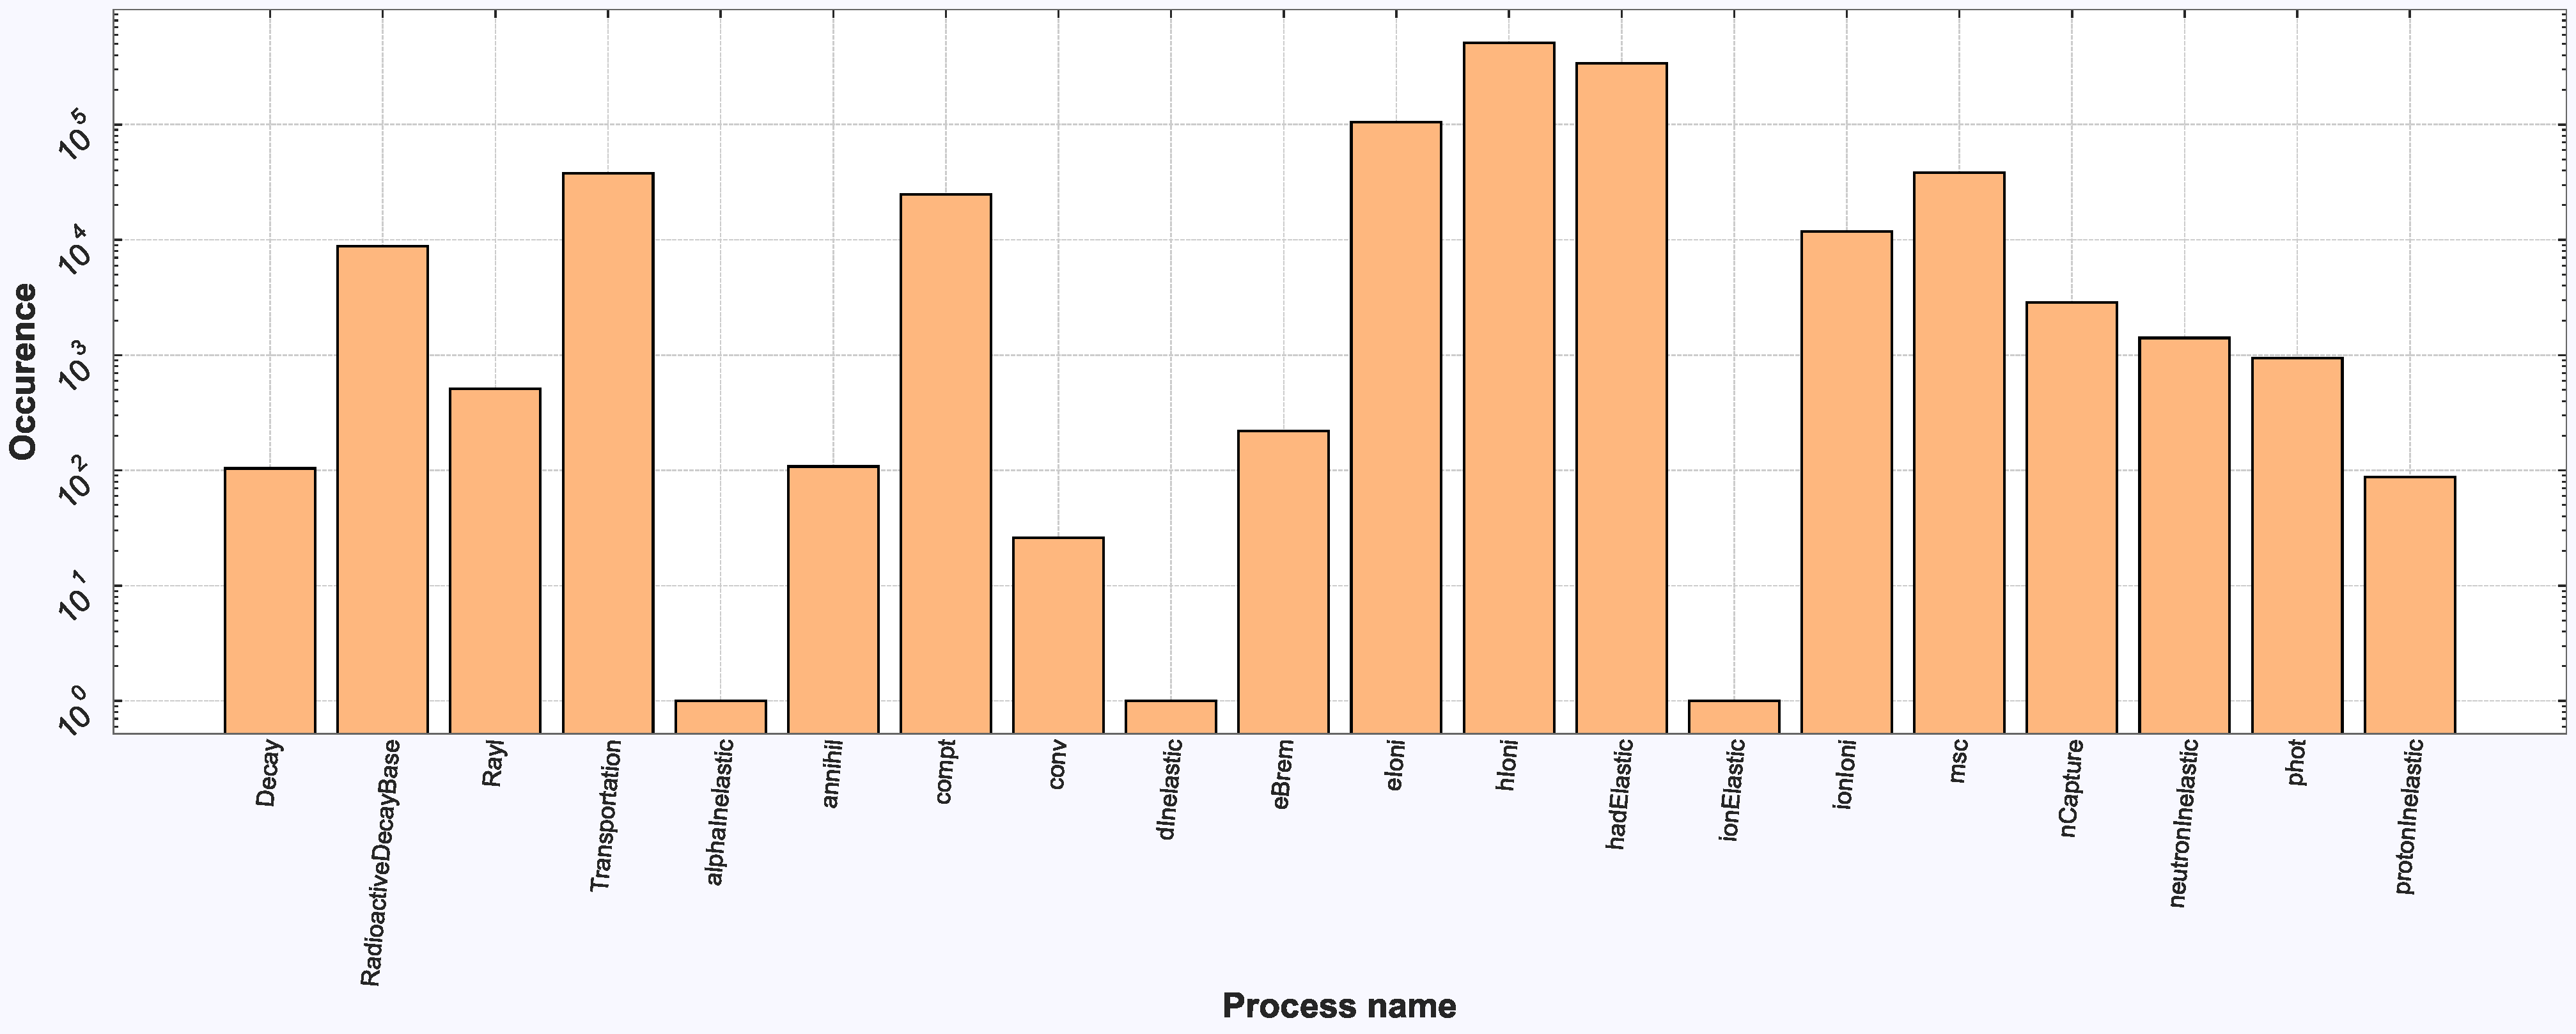
\includegraphics[clip,width=\textwidth]{{images/process_dist_E120_phQGSP_BIC_HP.pdf}}
}

\subfloat[Physics list used : \texttt{QGSP\_INCLXX\_HP}]{%
  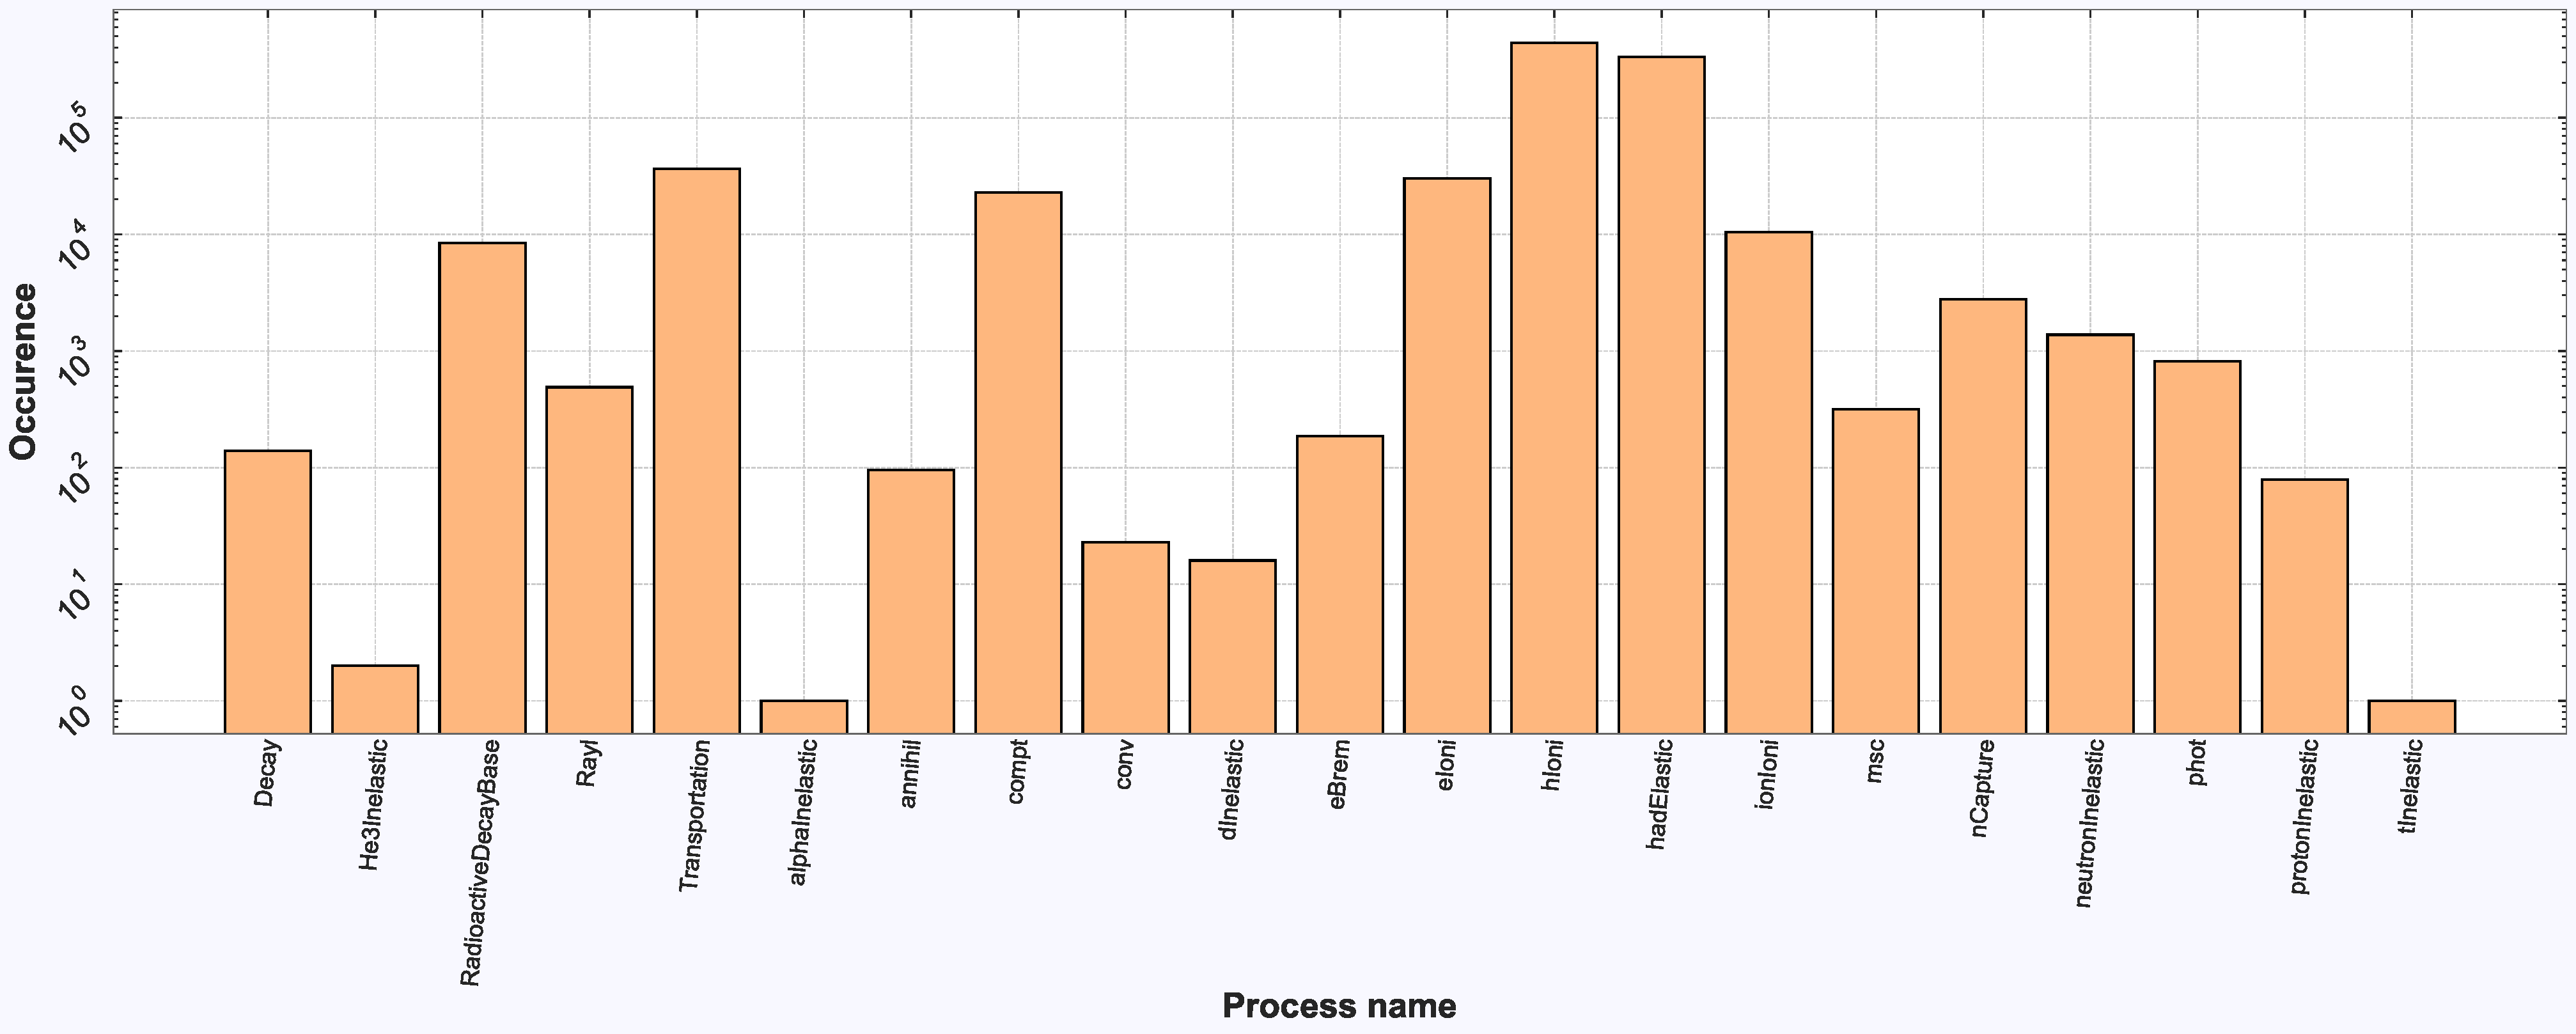
\includegraphics[clip,width=\textwidth]{{images/process_dist_E120_phQGSP_INCLXX_HP.pdf}}
}

\captionof{figure}{The number of steps with the given physical processes calculated during the simulation. On the X-axis the Geant4 shortenings of the processes can be seen.}\label{fig:5}
\end{figure}

\newpage

\begin{figure}[htp]
\subfloat[Physics list used : \texttt{QGSP\_BERT\_HP}]{%
  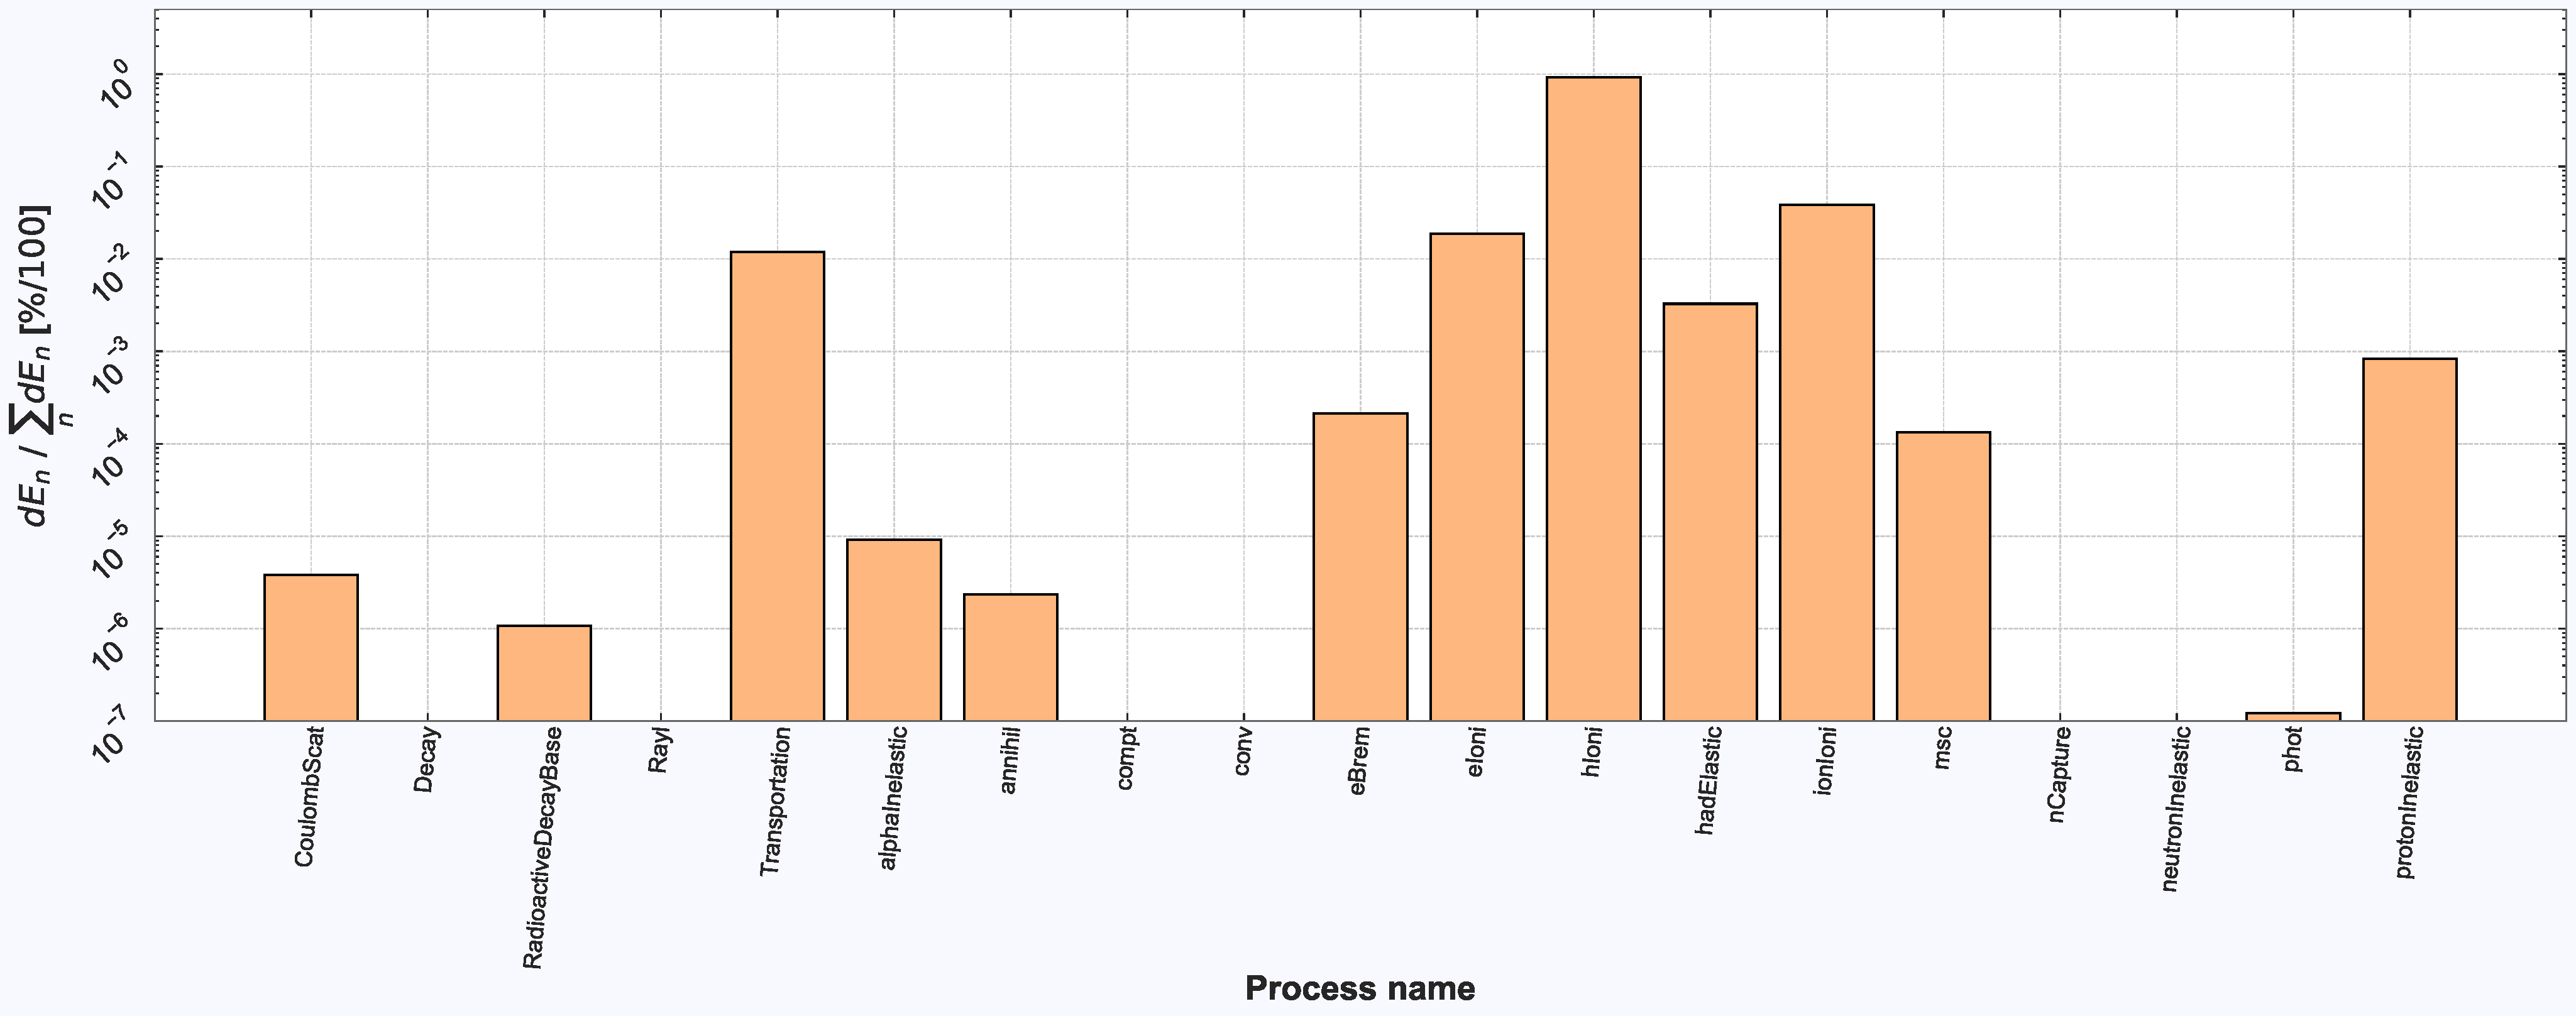
\includegraphics[clip,width=\textwidth]{{images/process_dist_weighted_E120_phQGSP_BERT_HP.pdf}}
}

\subfloat[Physics list used : \texttt{QGSP\_BIC\_HP}]{%
  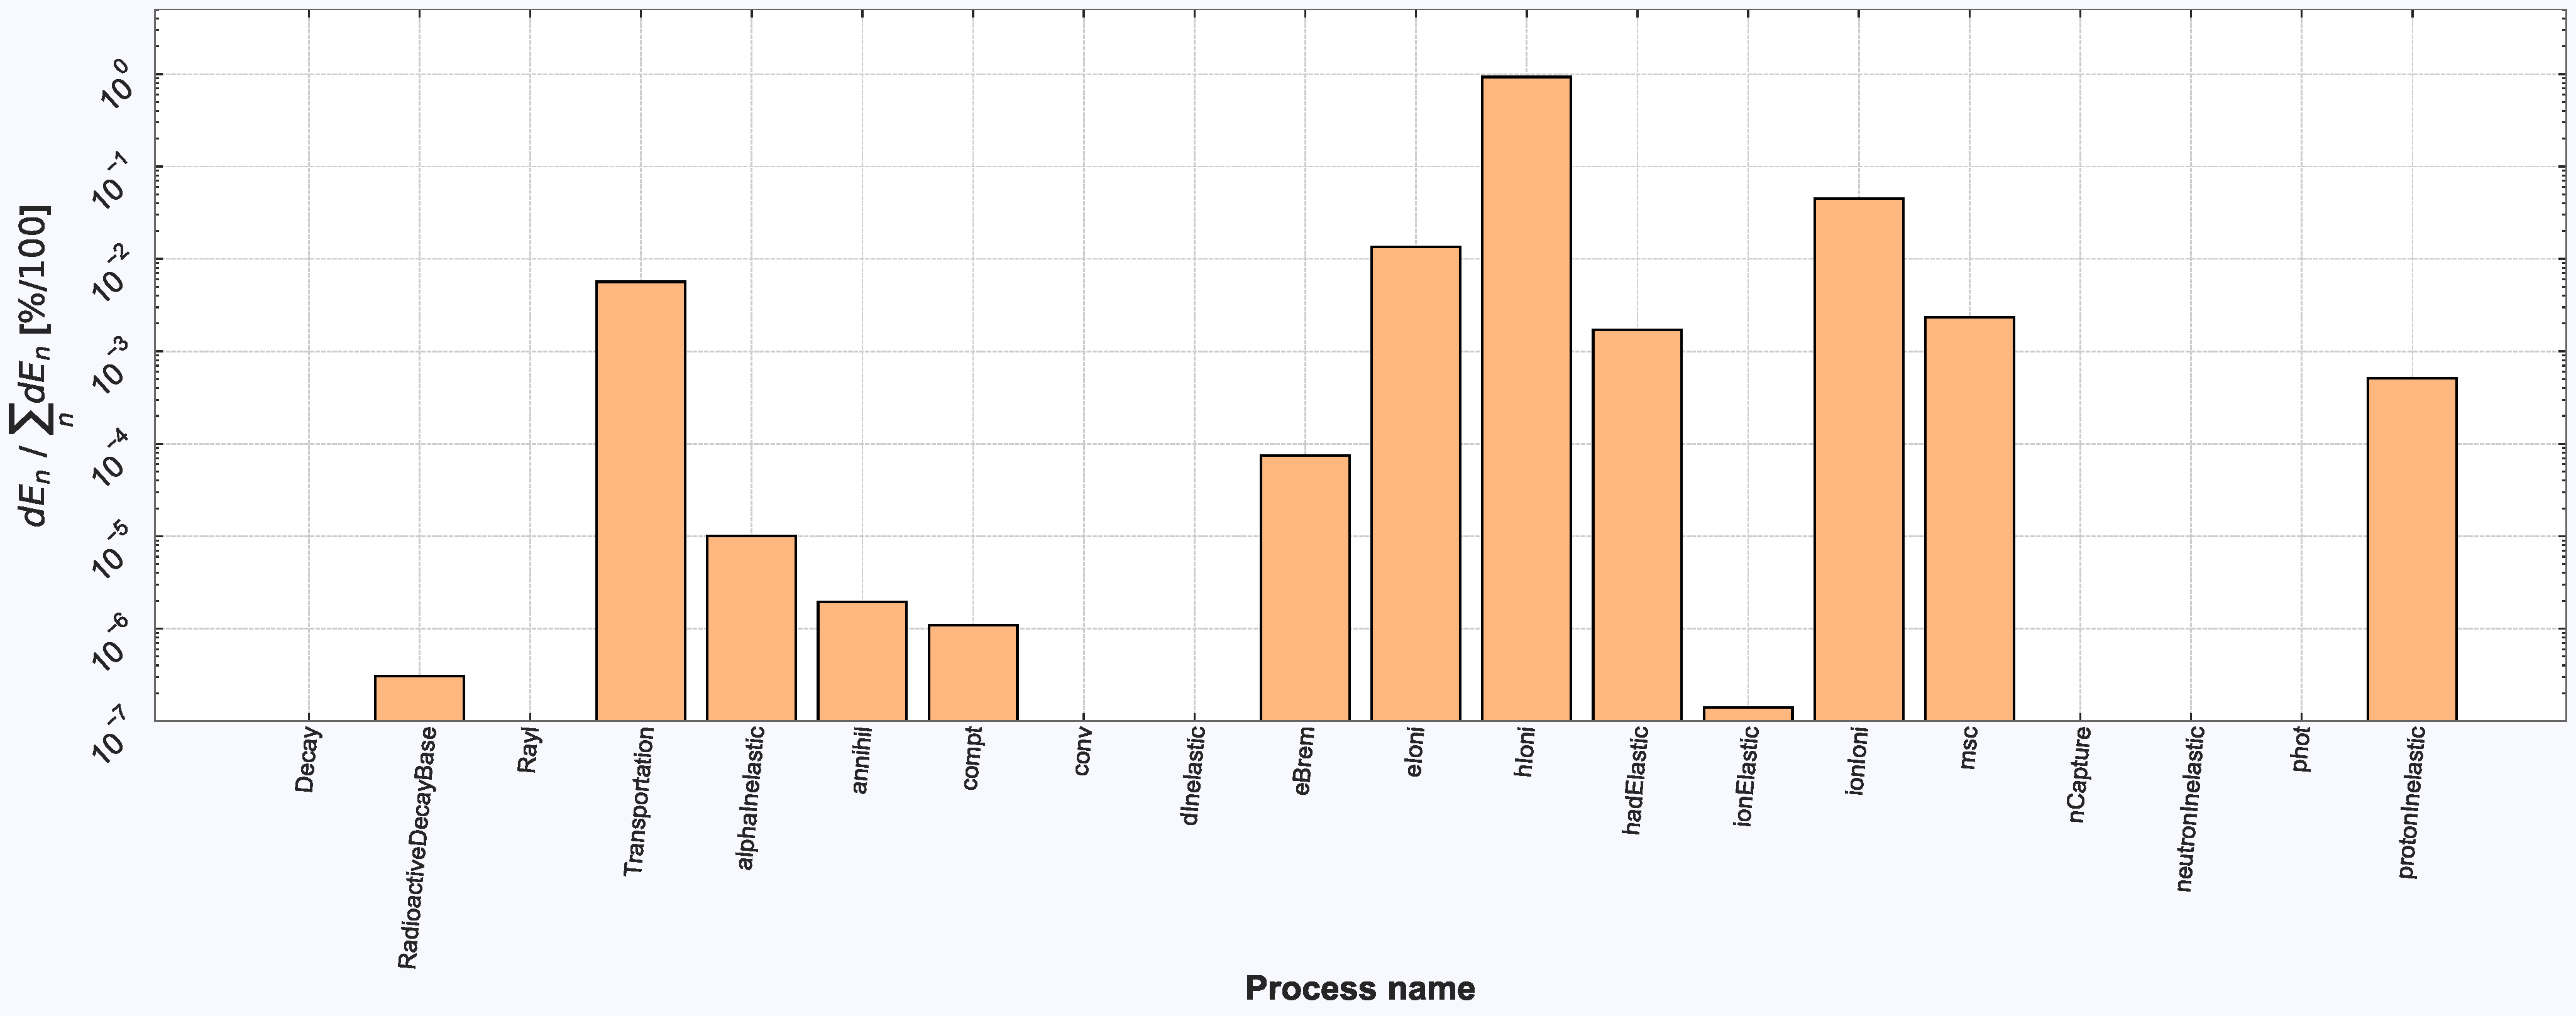
\includegraphics[clip,width=\textwidth]{{images/process_dist_weighted_E120_phQGSP_BIC_HP.pdf}}
}

\subfloat[Physics list used : \texttt{QGSP\_INCLXX\_HP}]{%
  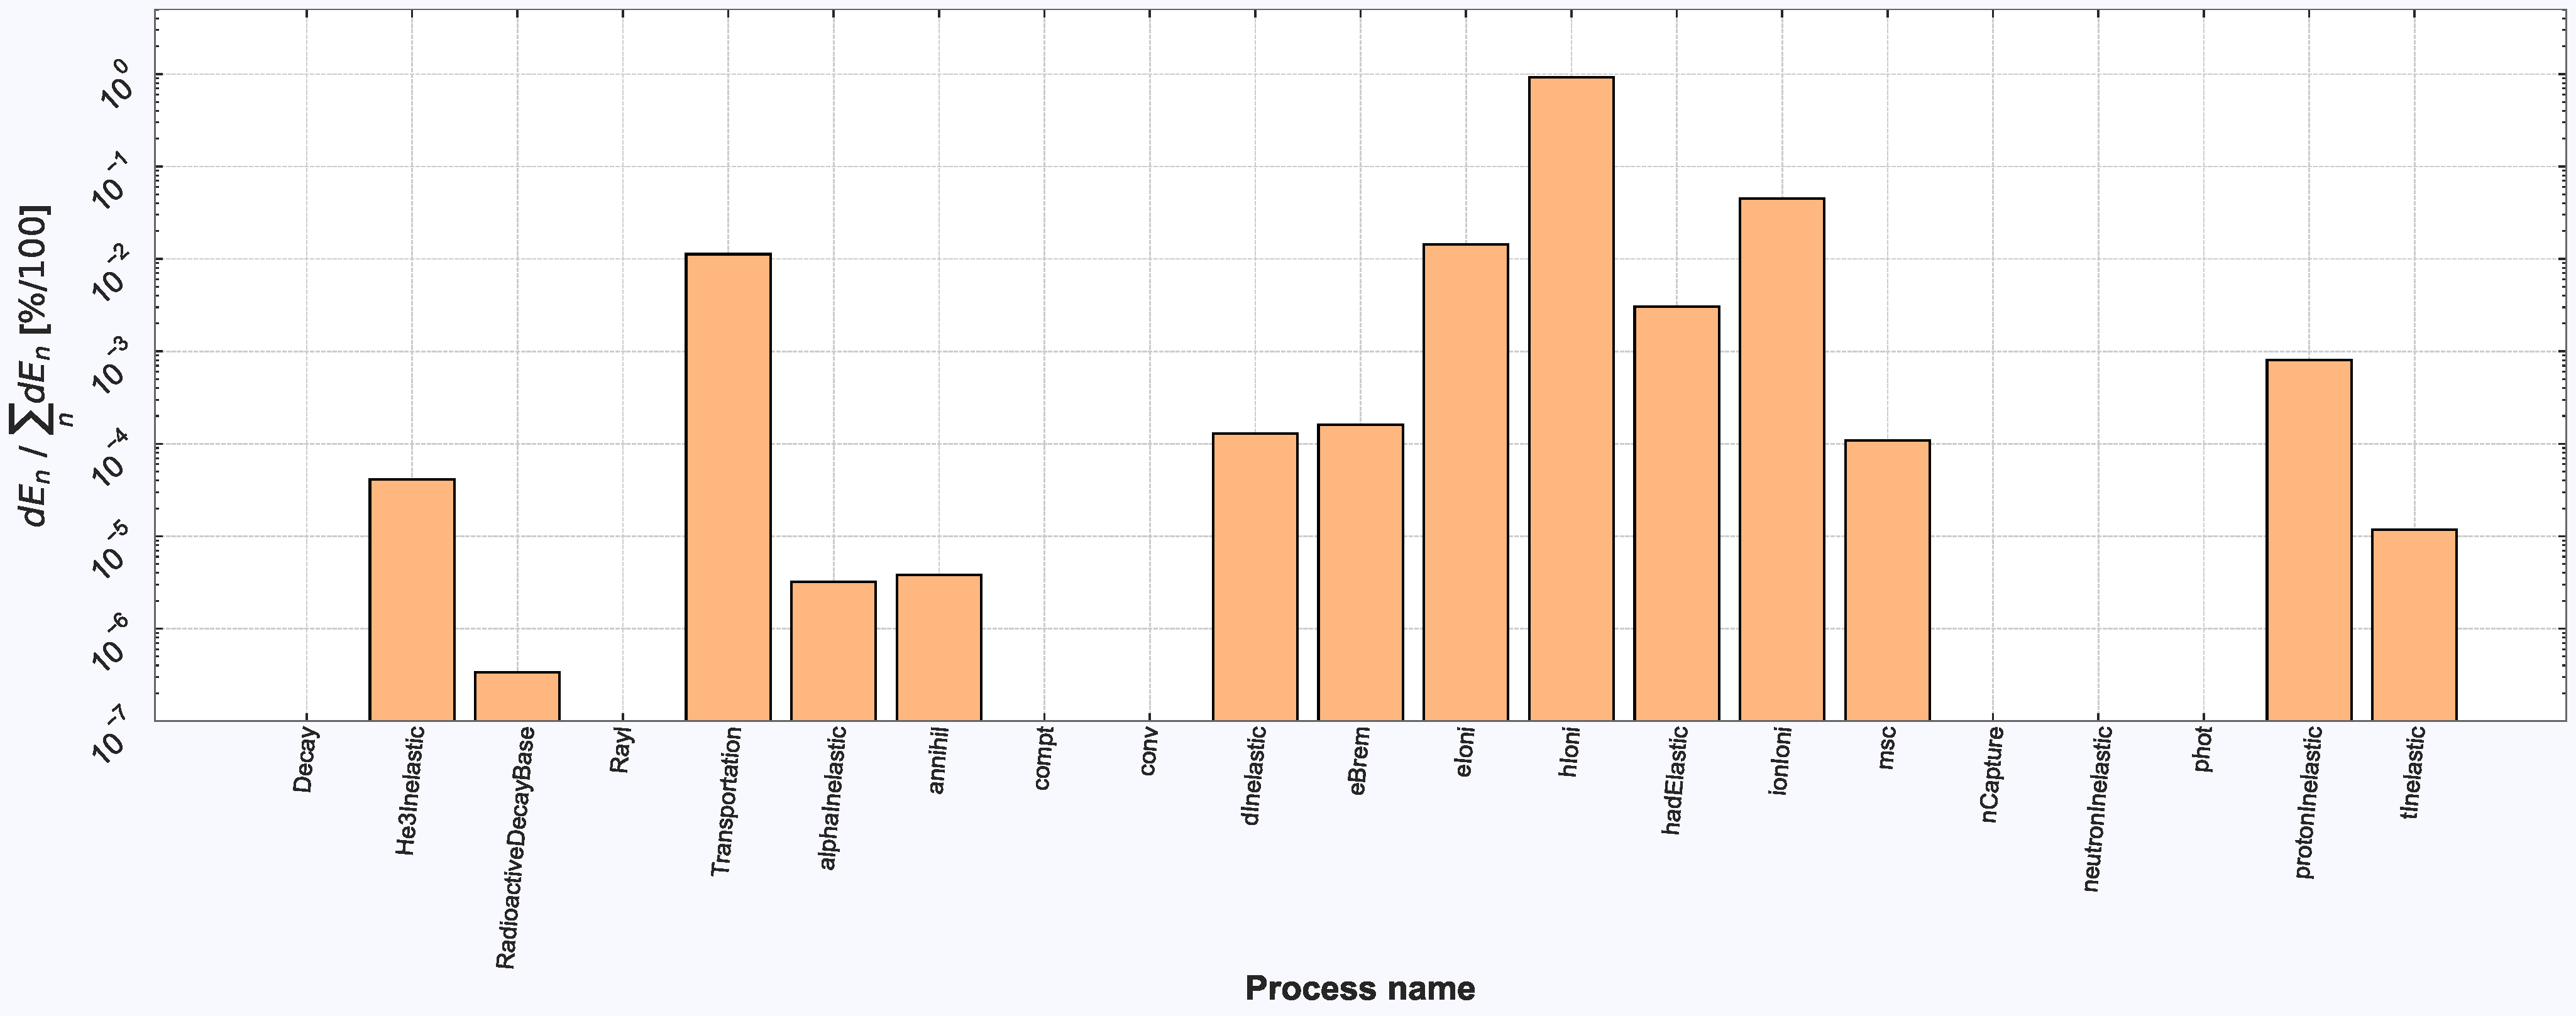
\includegraphics[clip,width=\textwidth]{{images/process_dist_weighted_E120_phQGSP_INCLXX_HP.pdf}}
}

\captionof{figure}{The number of steps with the given physical processes calculated during the simulation, weighted by the deposited energy during those processes. On the X-axis the Geant4 shortenings of the processes can be seen.}\label{fig:6}
\end{figure}

\newpage

\subsection{Particles}
\begin{figure}[htp]
\subfloat[Physics list used : \texttt{QGSP\_BERT\_HP}]{%
  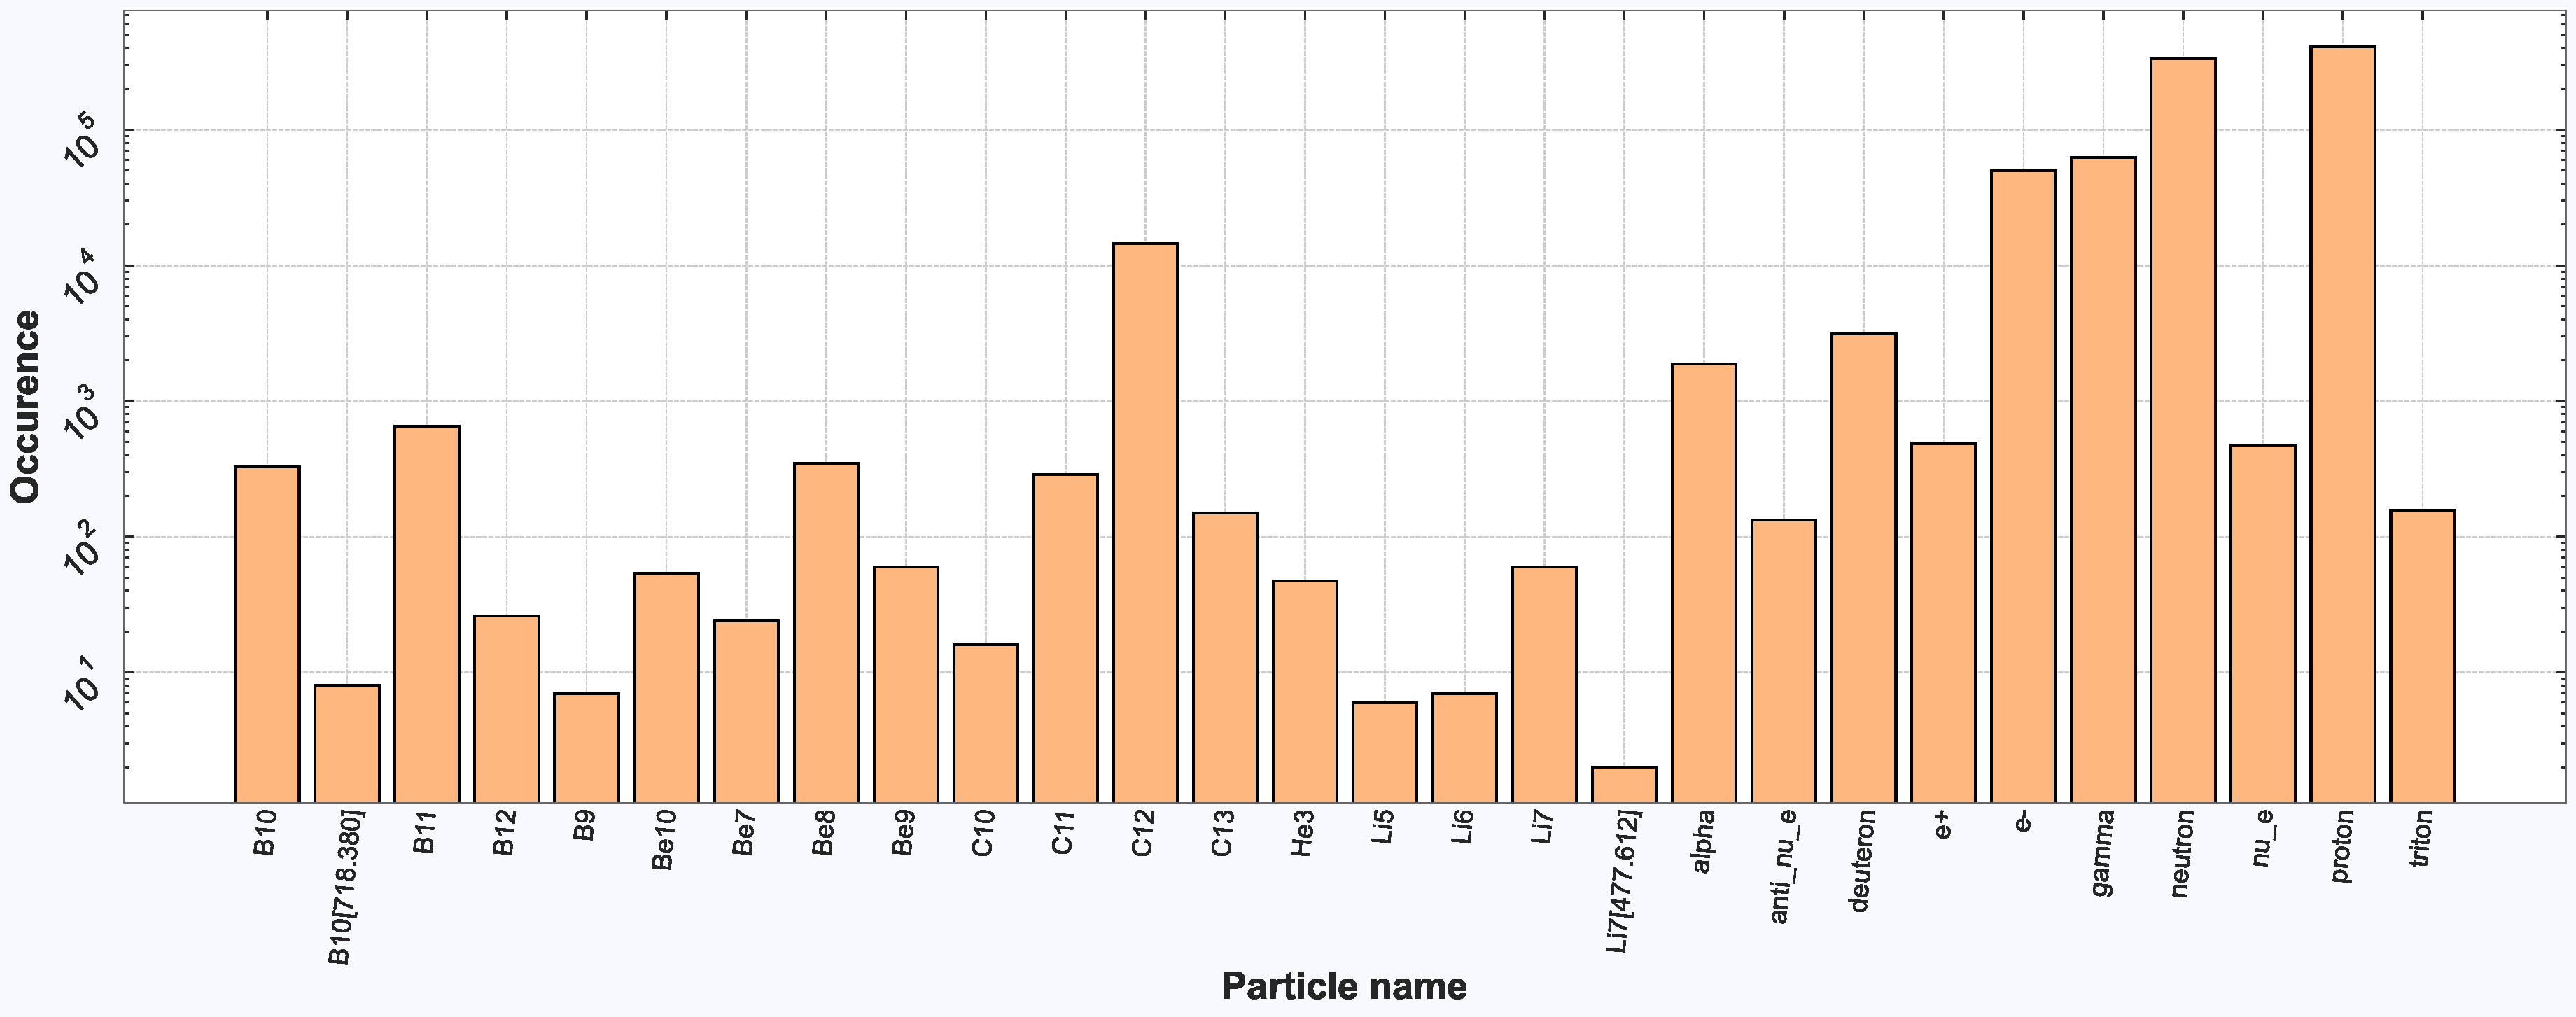
\includegraphics[clip,width=\textwidth]{{images/particle_dist_E120_phQGSP_BERT_HP.pdf}}
}

\subfloat[Physics list used : \texttt{QGSP\_BIC\_HP}]{%
  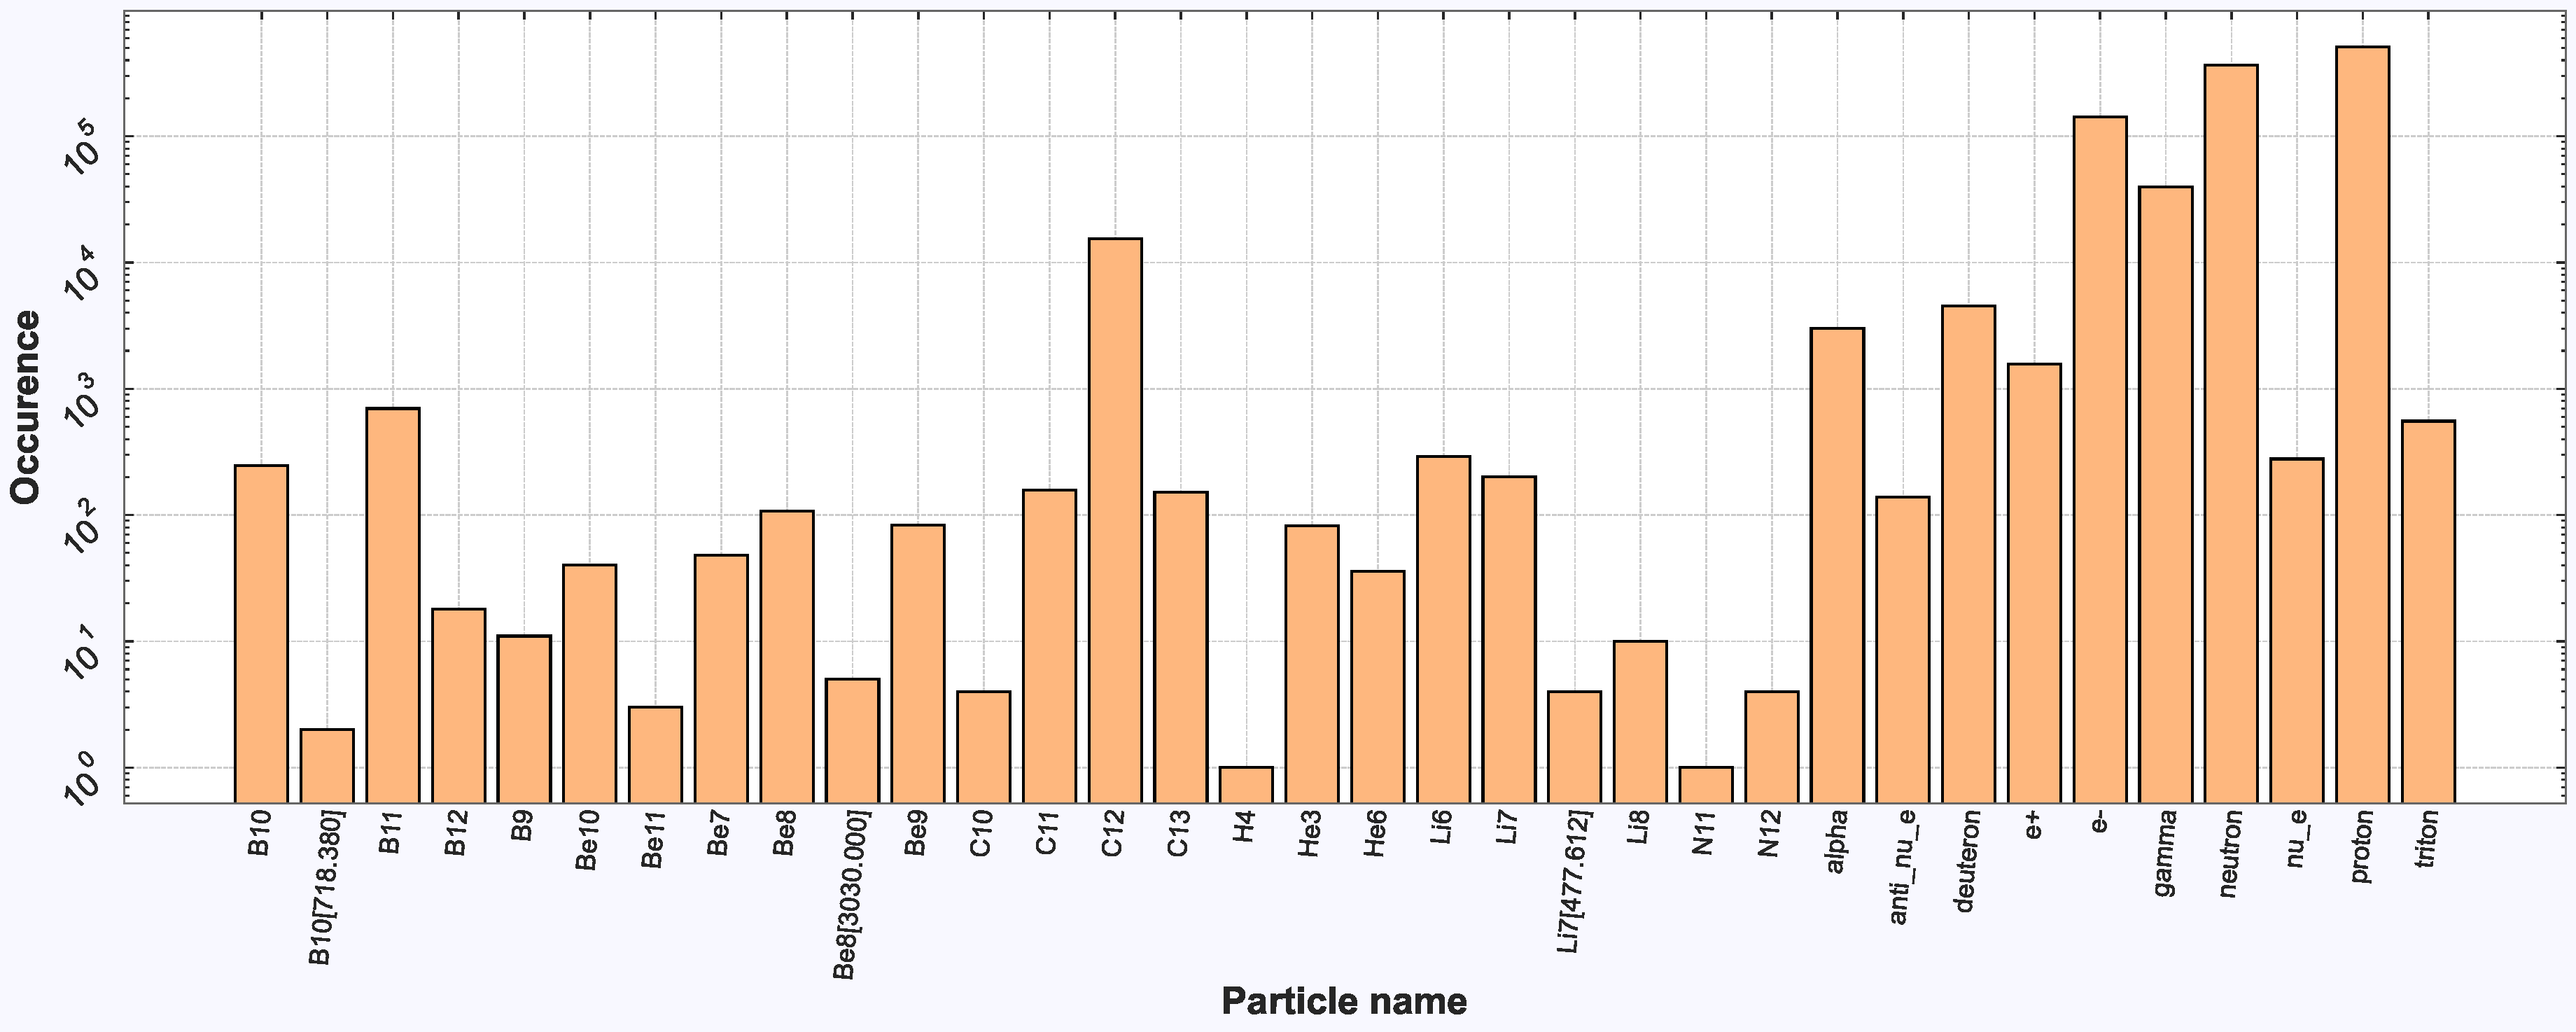
\includegraphics[clip,width=\textwidth]{{images/particle_dist_E120_phQGSP_BIC_HP.pdf}}
}

\subfloat[Physics list used : \texttt{QGSP\_INCLXX\_HP}]{%
  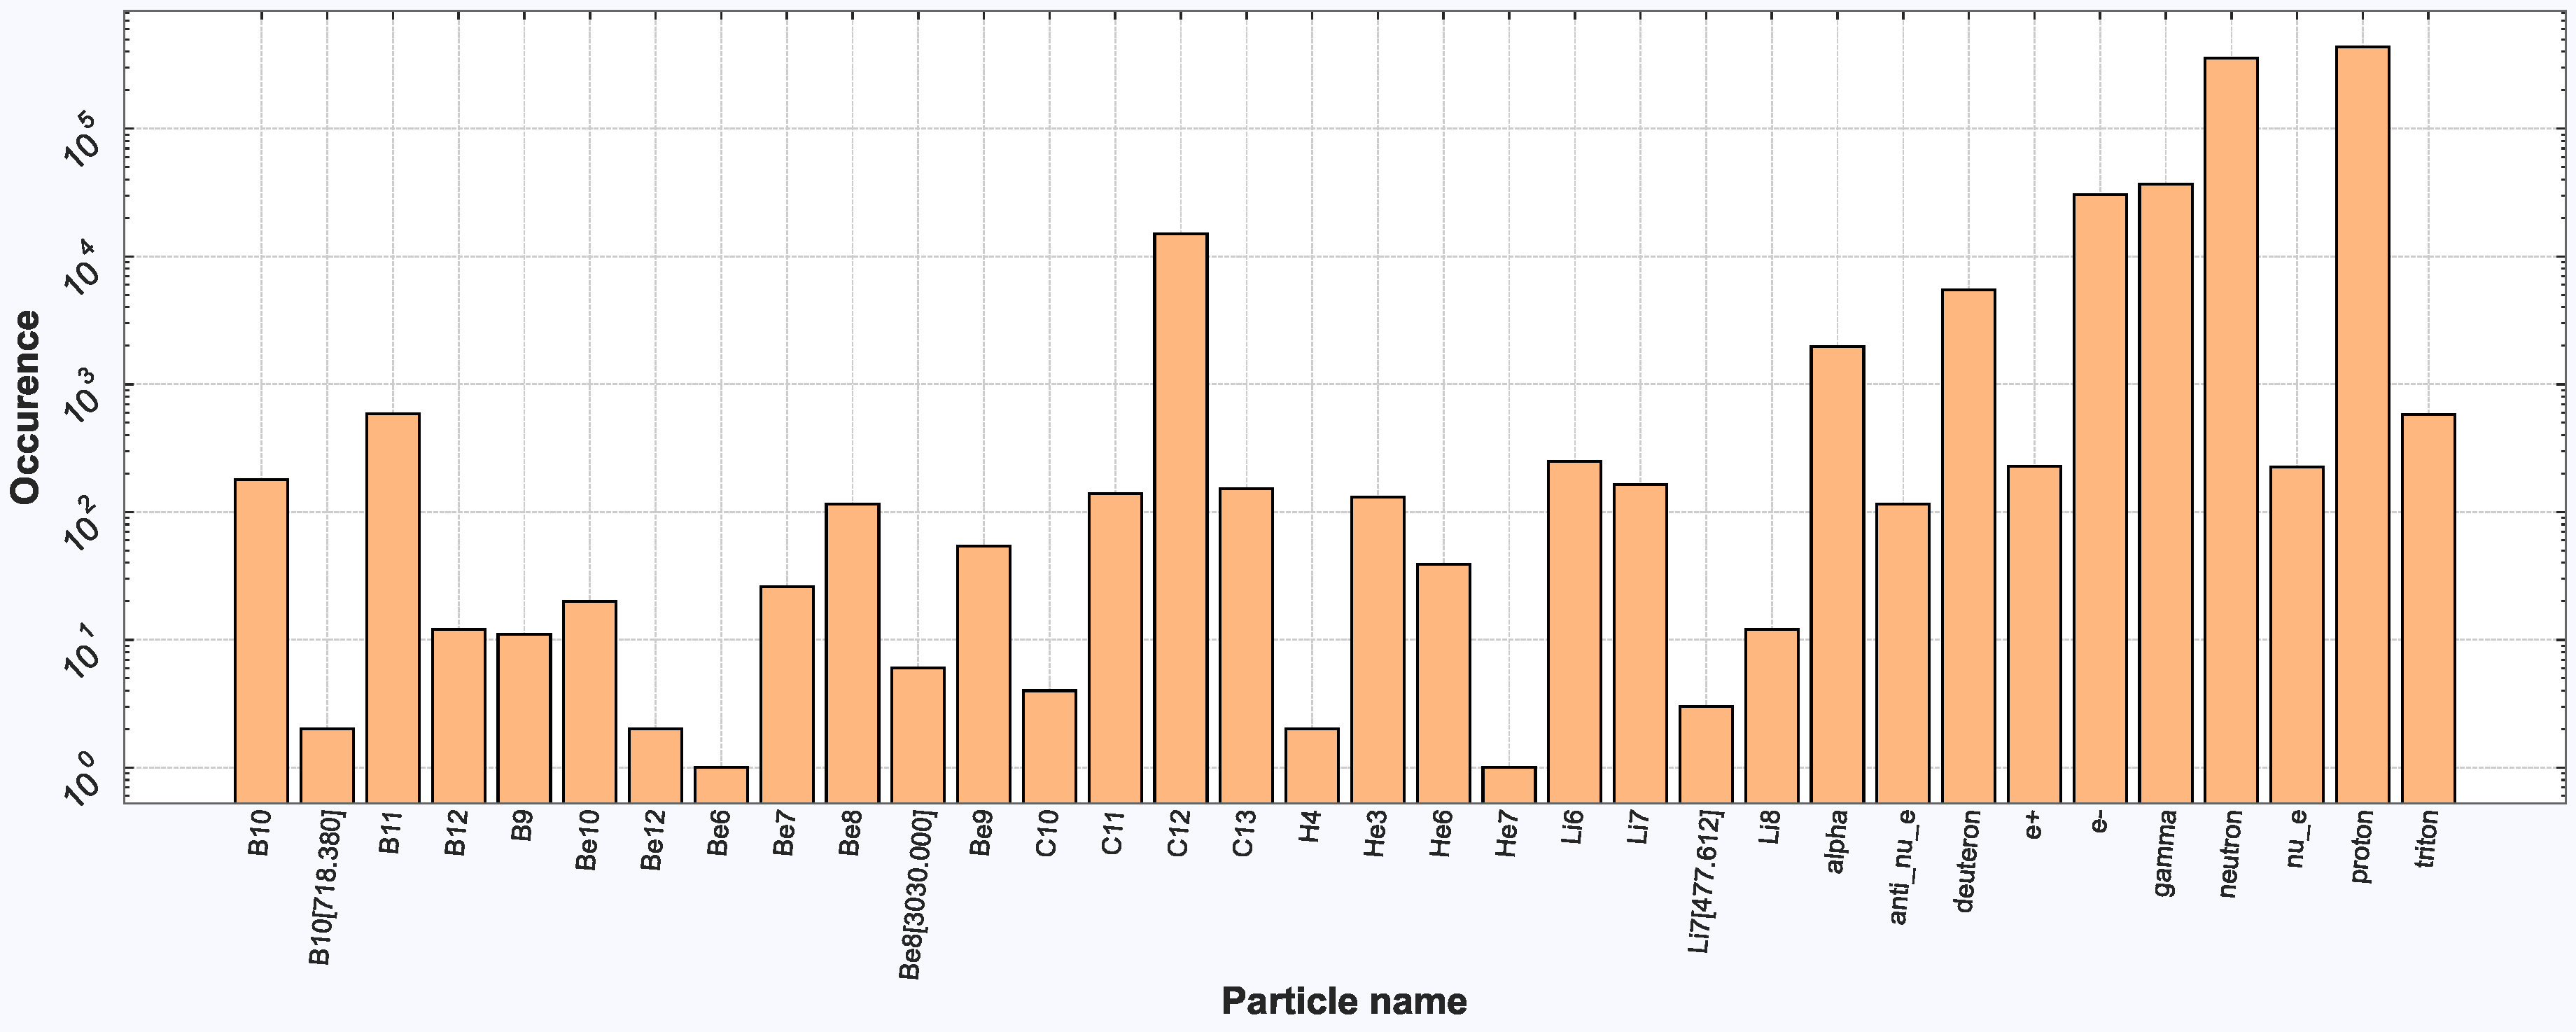
\includegraphics[clip,width=\textwidth]{{images/particle_dist_E120_phQGSP_INCLXX_HP.pdf}}
}

\captionof{figure}{The number of steps calculated by Geant4 for the given particle types. This figure just vaguely represents the actual number of particles of a given type taken place in the simulation.}\label{fig:7}
\end{figure}

\newpage

\begin{figure}[htp]
\subfloat[Physics list used : \texttt{QGSP\_BERT\_HP}]{%
  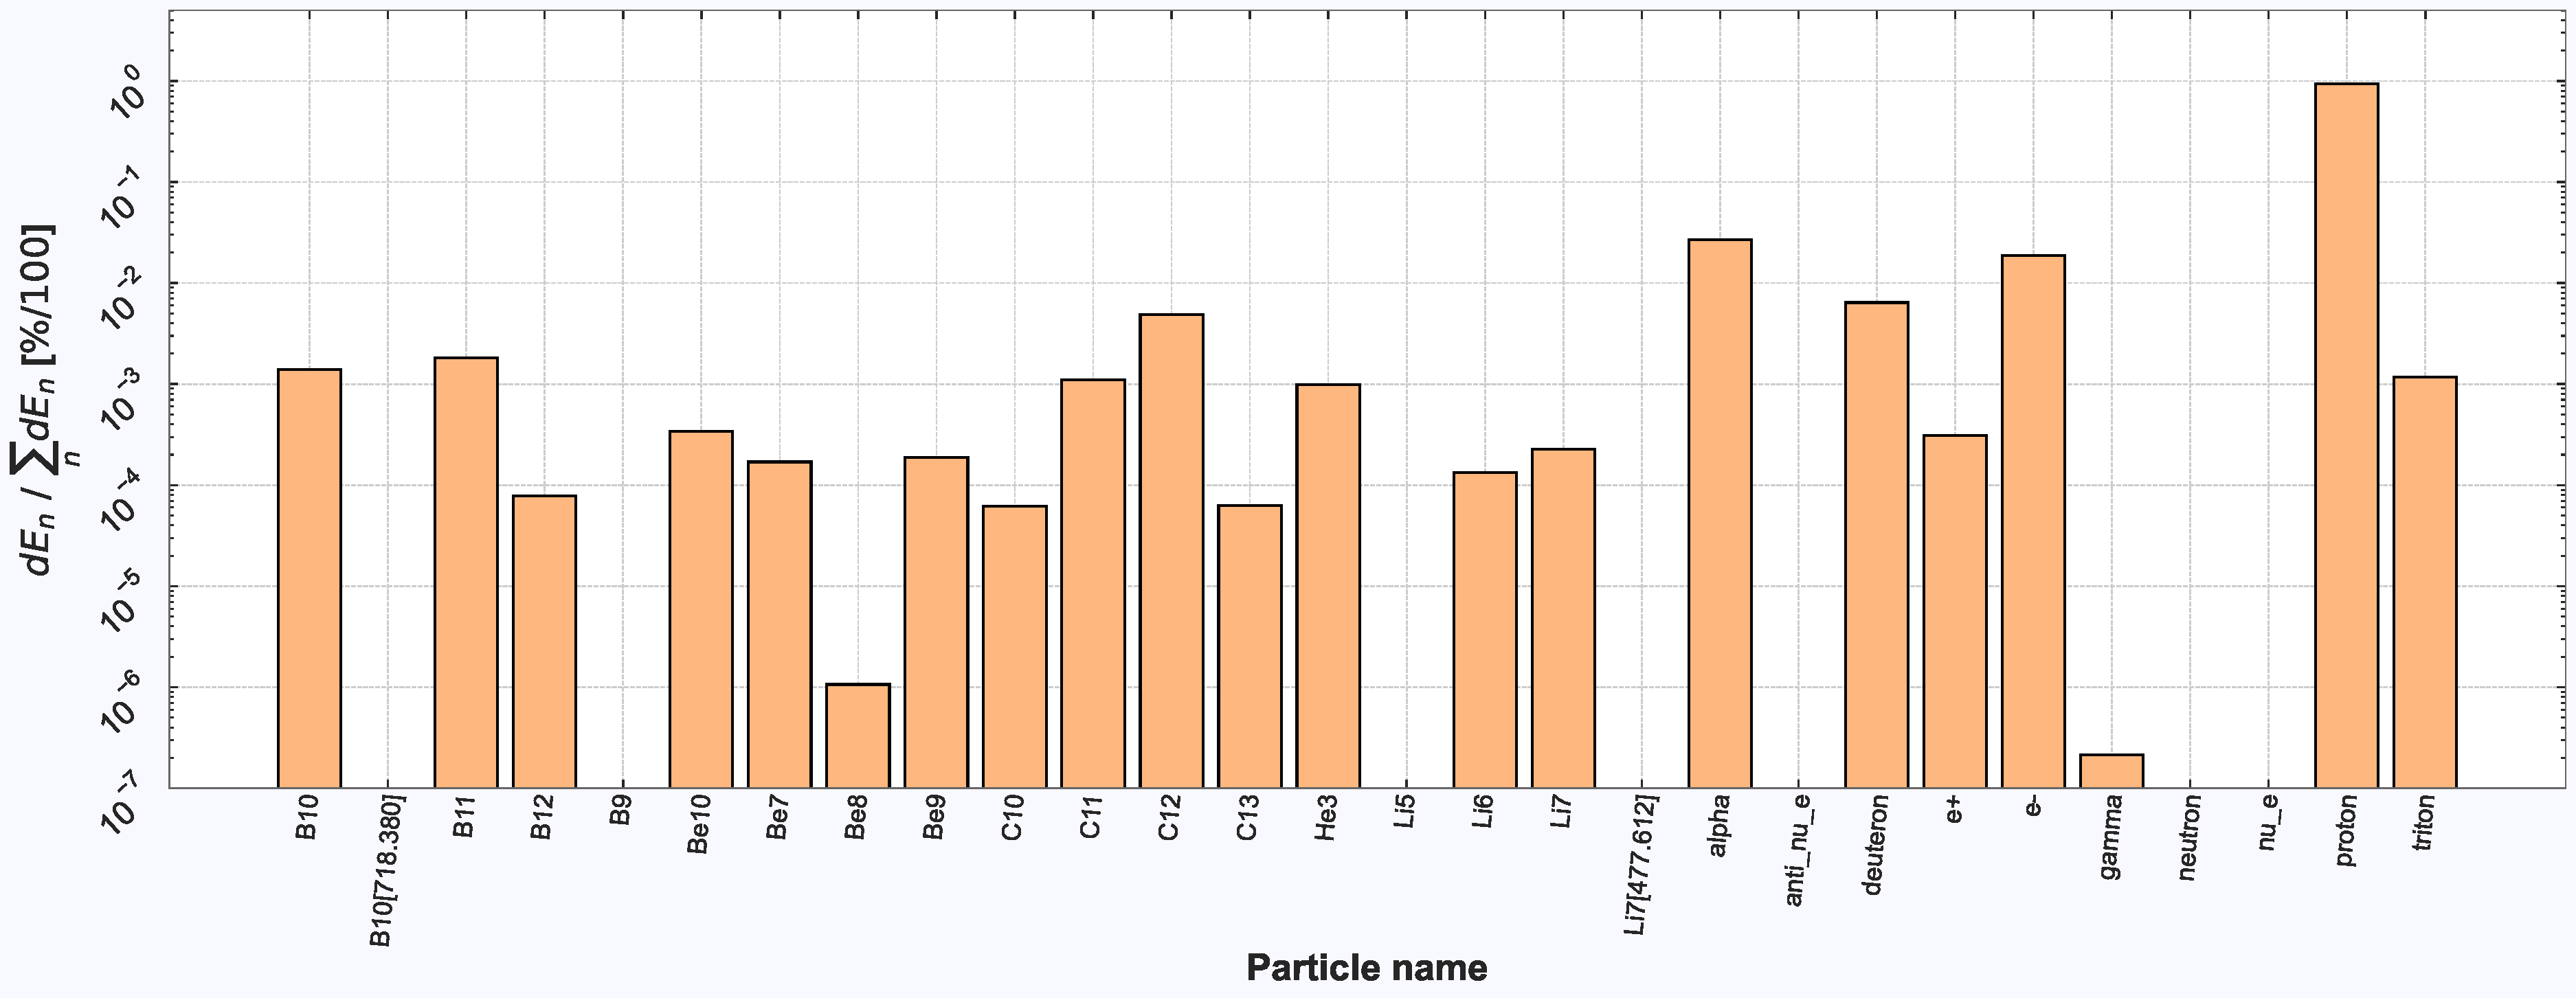
\includegraphics[clip,width=\textwidth]{{images/particle_dist_weighted_E120_phQGSP_BERT_HP.pdf}}
}

\subfloat[Physics list used : \texttt{QGSP\_BIC\_HP}]{%
  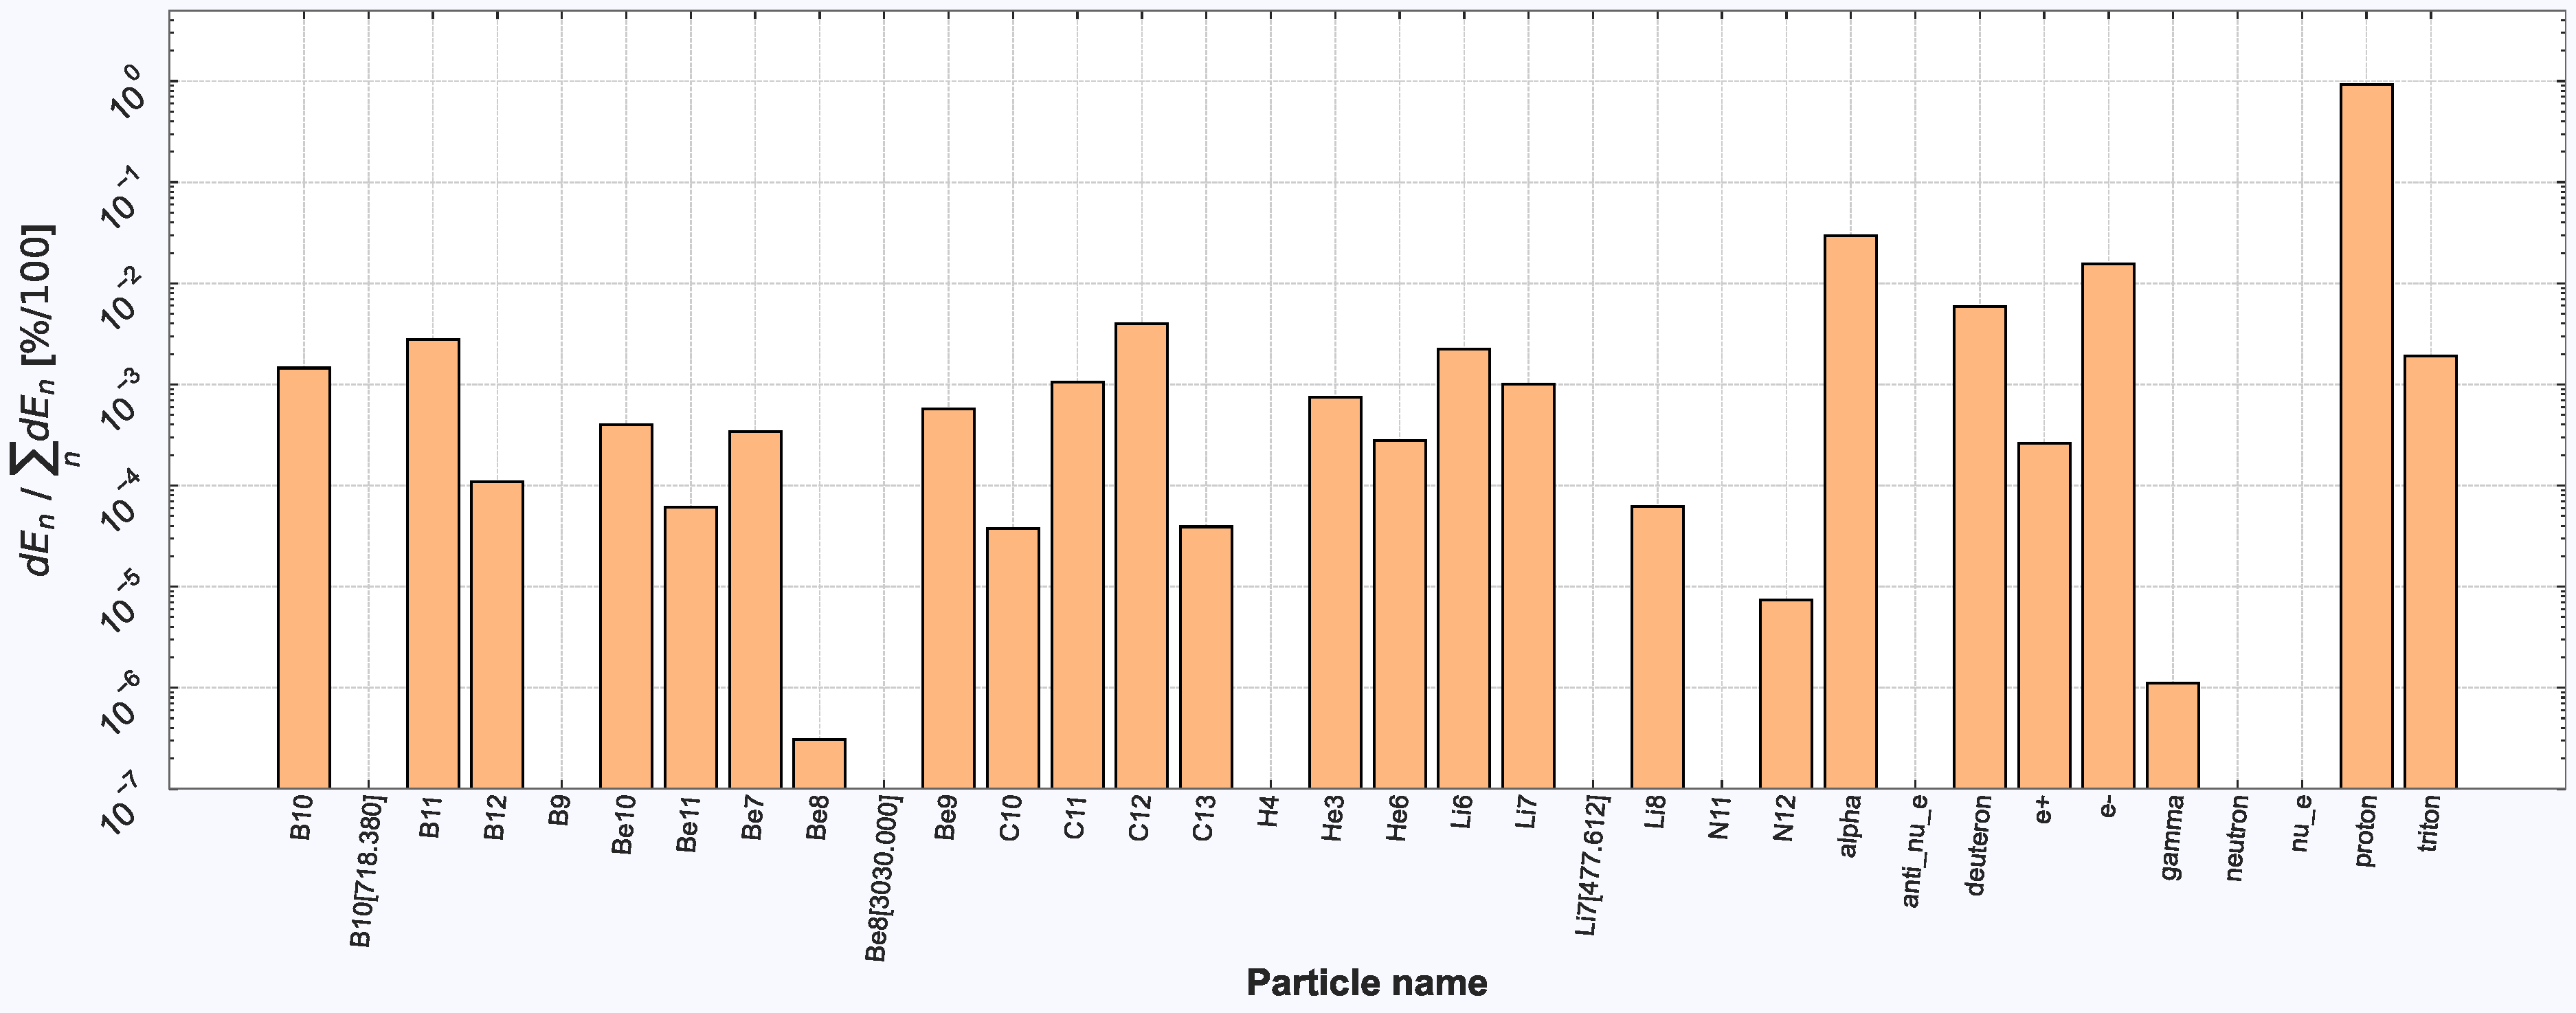
\includegraphics[clip,width=\textwidth]{{images/particle_dist_weighted_E120_phQGSP_BIC_HP.pdf}}
}

\subfloat[Physics list used : \texttt{QGSP\_INCLXX\_HP}]{%
  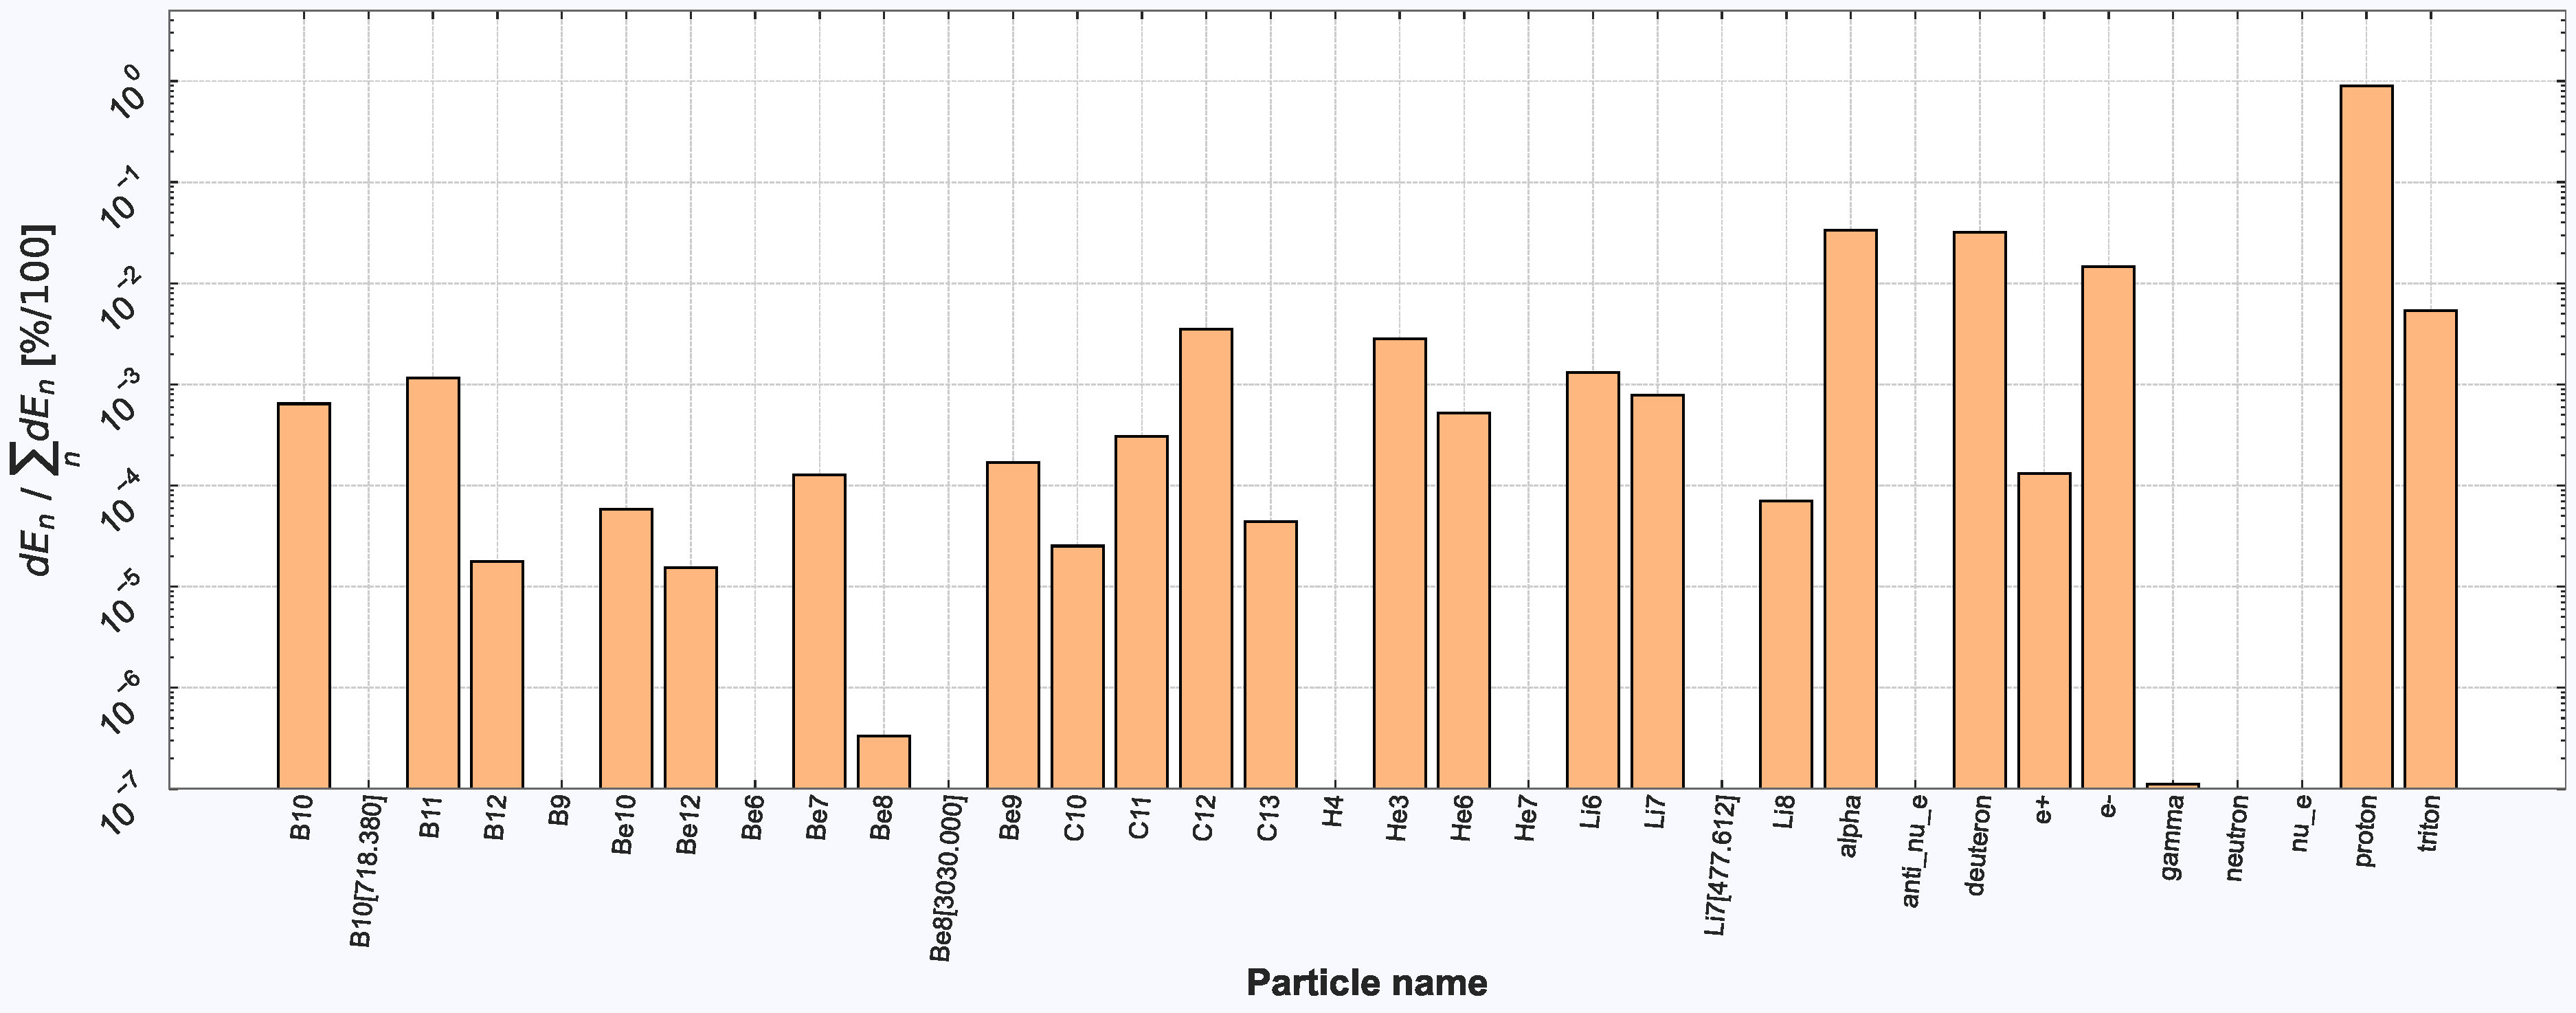
\includegraphics[clip,width=\textwidth]{{images/particle_dist_weighted_E120_phQGSP_INCLXX_HP.pdf}}
}

\captionof{figure}{The number of steps calculated by Geant4 for the given particle types. This figure just vaguely represents the actual number of particles of a given type taken place in the simulation.}\label{fig:8}
\end{figure}

\newpage

\subsection{Detection accuracy}
\begin{figure}[h]
	\captionsetup{justification=centering}
	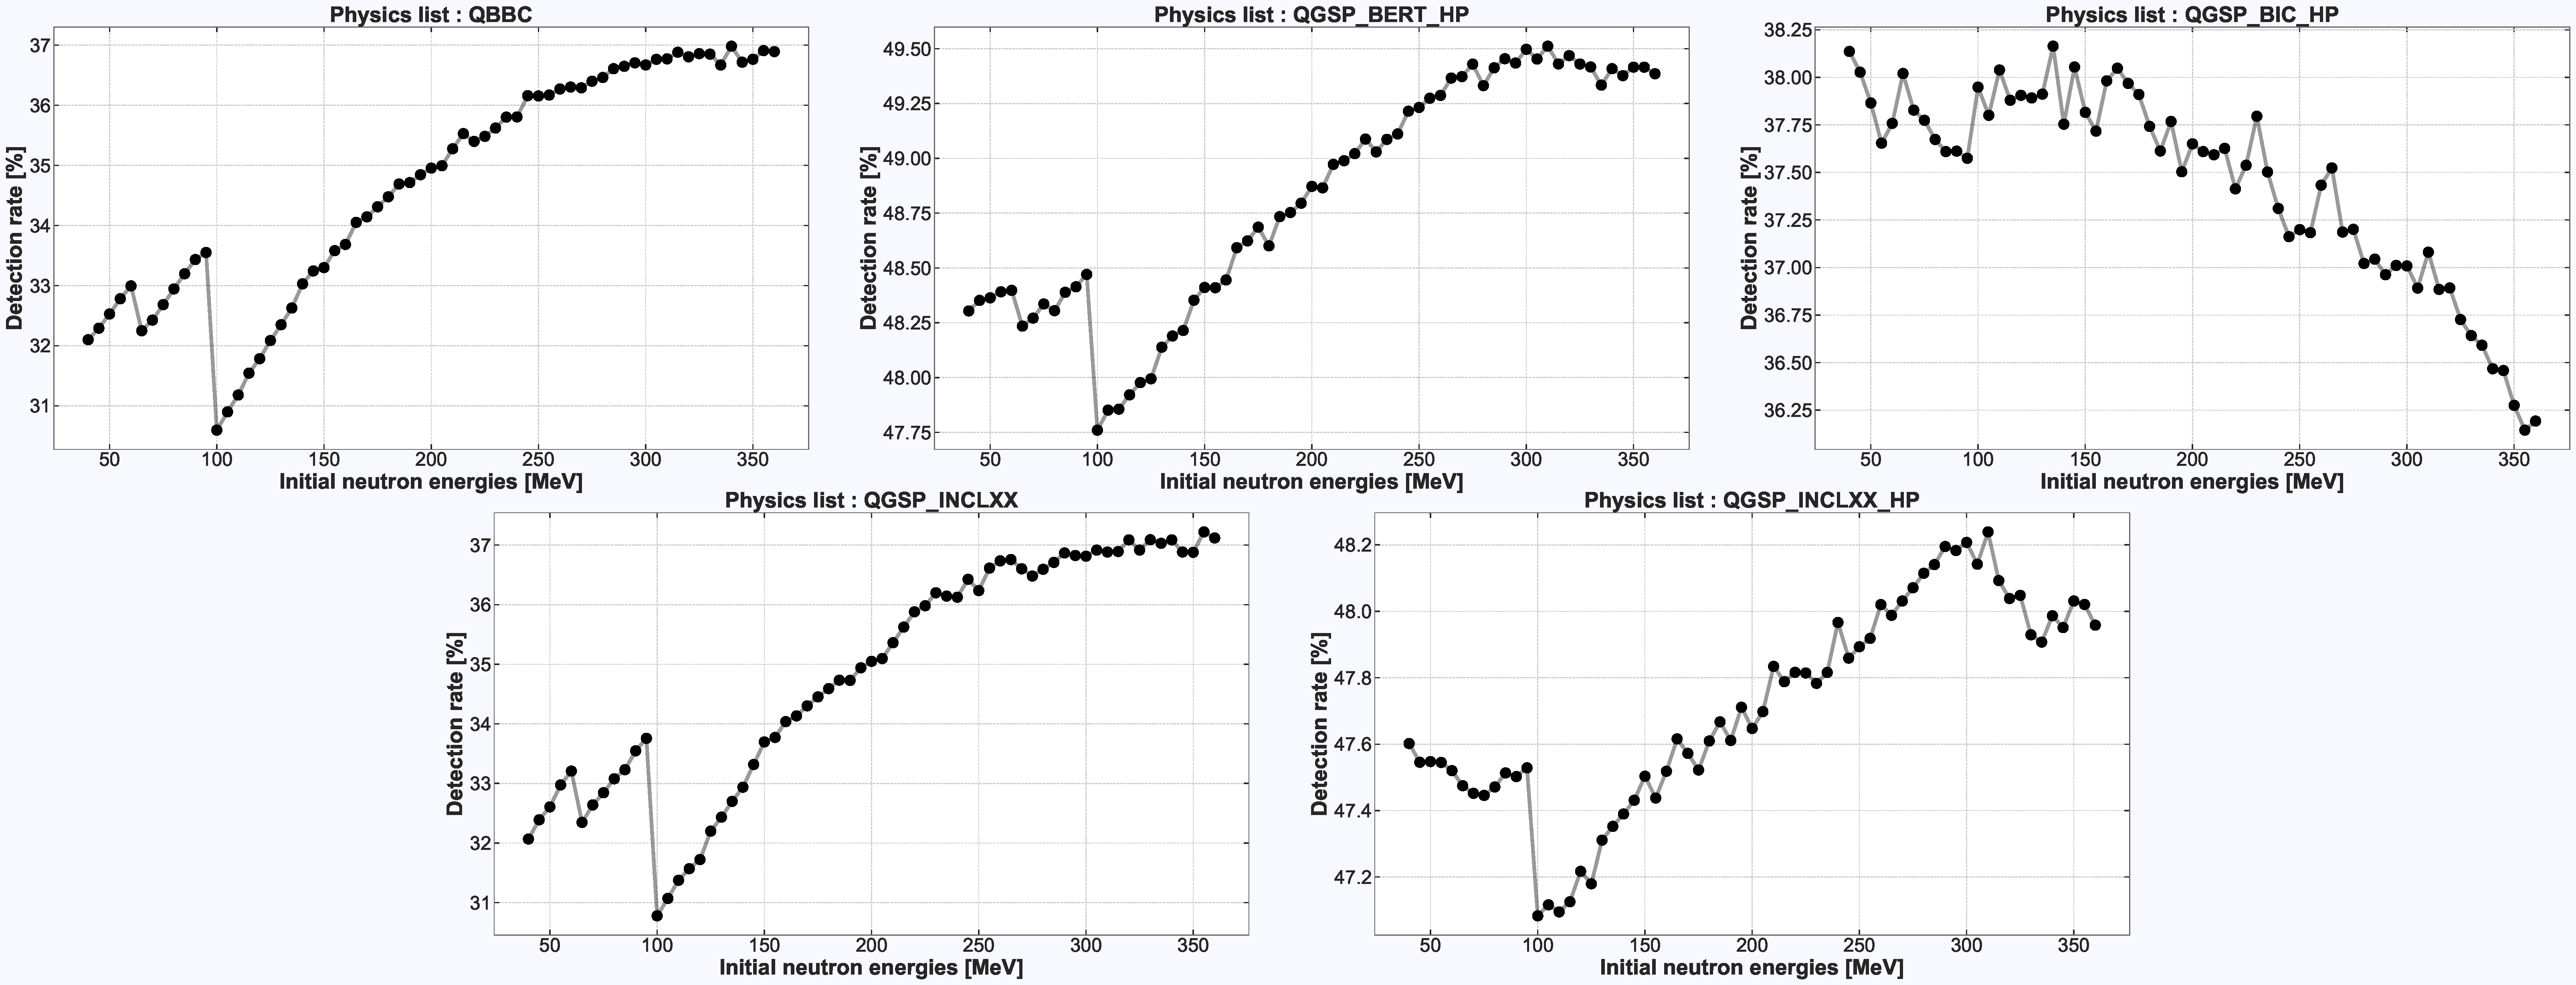
\includegraphics[width=\textwidth]{{images/detection_rates.pdf}}
	\captionof{figure}{Detection accuracy of particle steps in the \texttt{NEUT} detector rods for all energy deposits.}\label{fig:9}
\end{figure}
\begin{figure}[h]
	\captionsetup{justification=centering}
	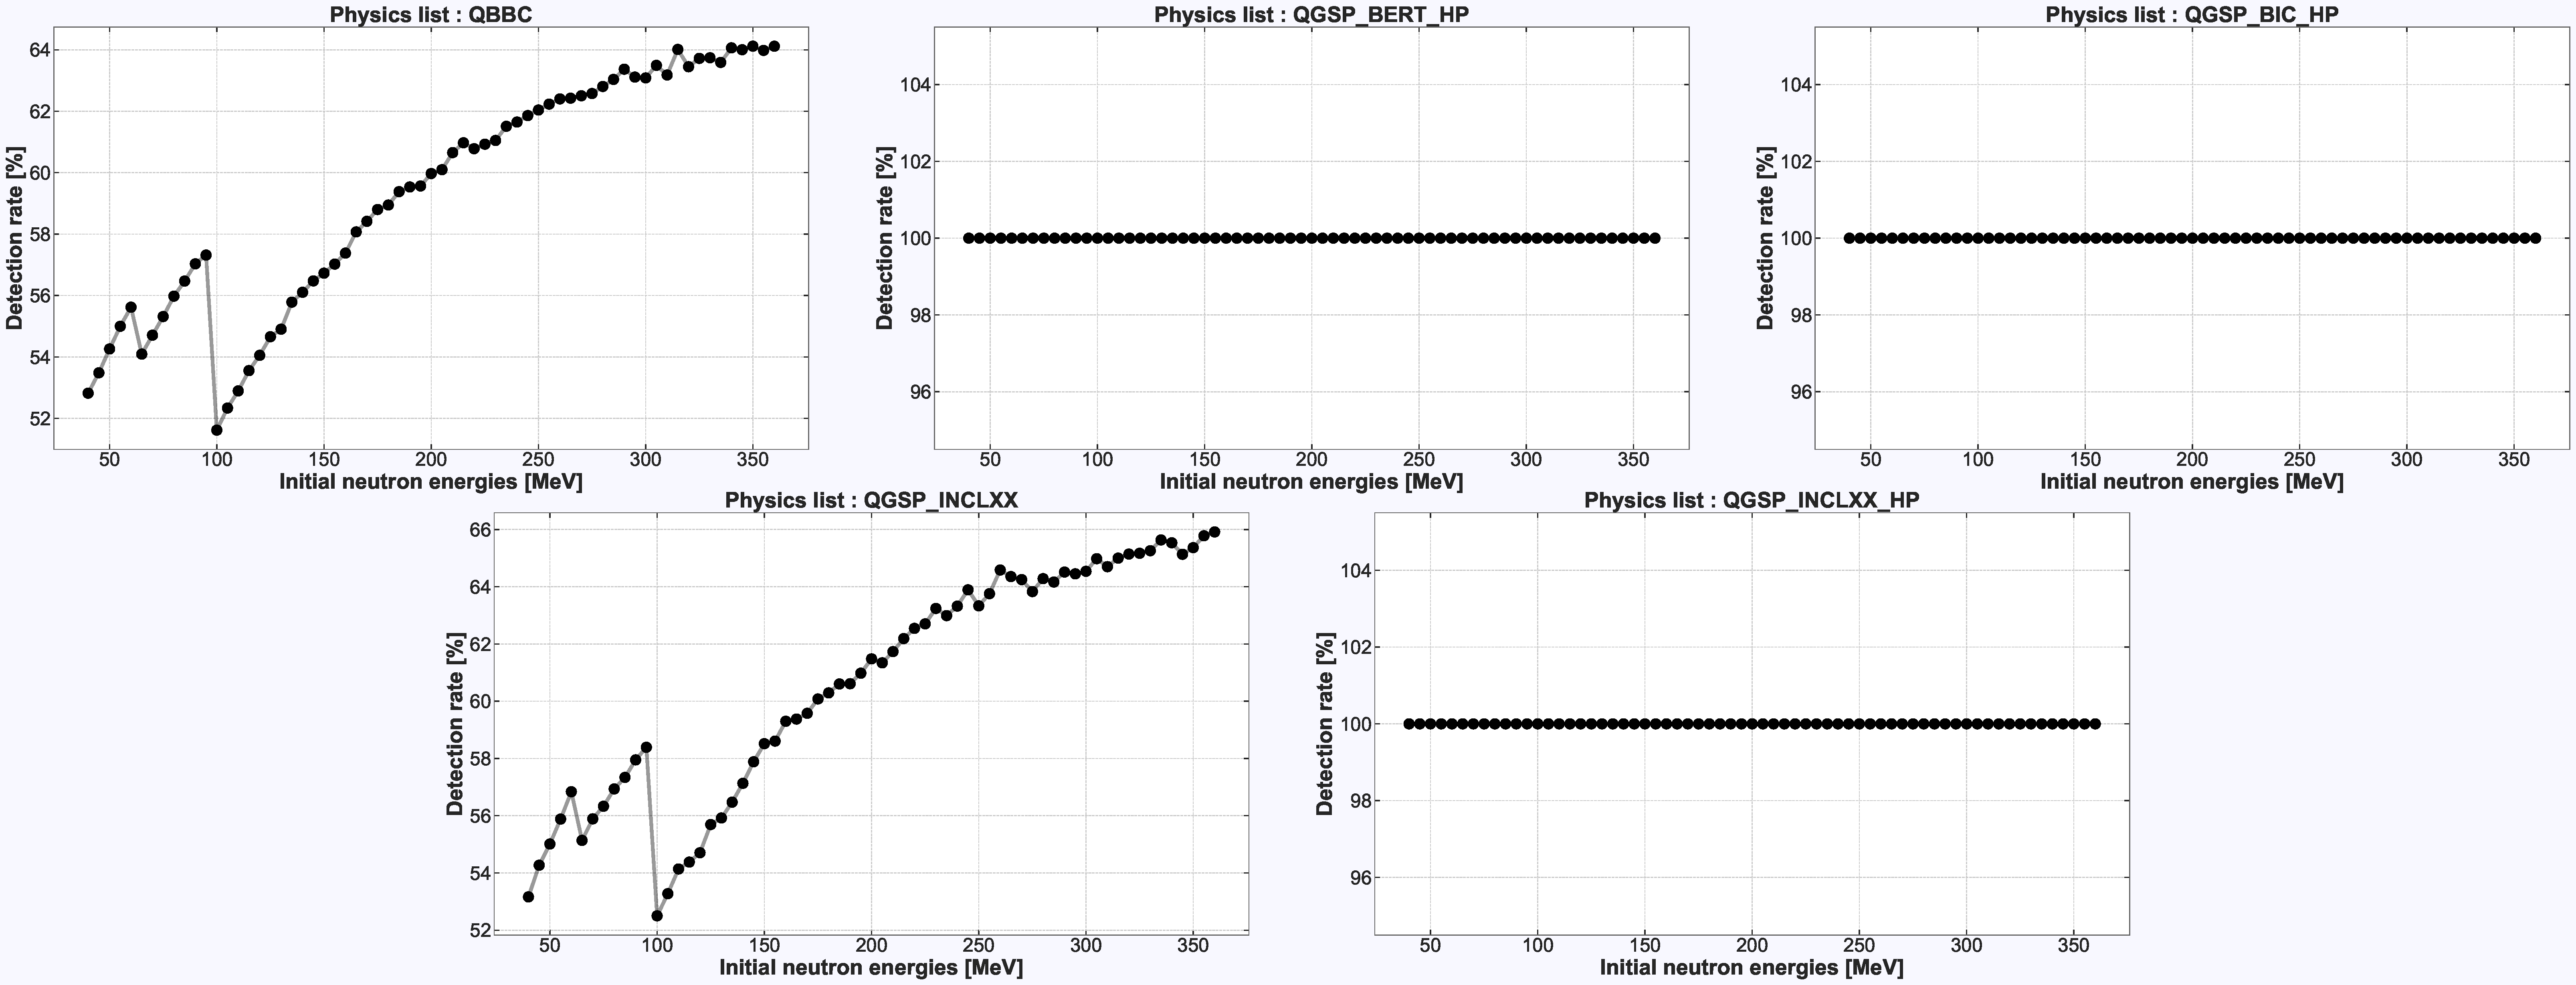
\includegraphics[width=\textwidth]{{images/detection_rates_neutron_only.pdf}}
	\captionof{figure}{Detection accuracy of particle steps in the \texttt{NEUT} detector rods for ONLY NEUTRON energy deposits.}\label{fig:10}
\end{figure}